 %\documentclass[prd,nofootinbib,floatfix,12pt,notitlepage,eqsecnum]{revtex4-1}
%%%%%%%%%%%%%%%%%%%%%%%%%%%%%%%%%%%%%%%%%%%%%%%%%%%%%%%%%%%%%%%%%%%%%%%%%%%%%%%%%%%%%%%%%%%%%%%%%%%%%%%%%%%%%%%%%%%%%%%%%%%%%%%%%%%%%%%
\documentclass[11pt]{article}

\usepackage{NotesTeX} %/Path/to/package should be replaced with package location
\usepackage{lipsum}
\usepackage{tensor}
\usepackage{graphicx,wrapfig,float,slashed,subcaption,bbold,bm}
\usepackage{amsmath,mathtools,amssymb,epsfig,graphicx,xcolor}
\usepackage{epstopdf}
\epstopdfsetup{update}
\usepackage{ragged2e}
\usepackage{mciteplus}
\usepackage[many]{tcolorbox}
\usepackage{pgfplots}
\pgfplotsset{compat=1.5.1}
\usepackage{tikz}
\usetikzlibrary{babel}
\tikzset{>=latex}
\usepackage{hyperref}

\newcommand{\bs}{\textbackslash}
\newcommand{\nc}{\newcommand}
\nc{\non}{\nonumber}	
\nc{\noi}{\noindent}
\nc{\barx}{\bar{x}}
%

\nc{\hsp}{\hspace{0.5cm}}
\nc{\lsp}{\hspace{1cm}}
\nc{\Lsp}{\hspace{2cm}}
\nc{\LLsp}{\lsp\lsp}
\nc{\lra}{\longrightarrow}
\nc{\p}{\prime}
\nc{\sgn}{\text{sgn}}
\nc{\ph}{\varphi}


\nc{\beq}{\begin{equation}}  \nc{\eeq}{\end{equation}}
\nc{\bea}{\begin{eqnarray}}  \nc{\eea}{\end{eqnarray}}
\nc{\baa}{\begin{array}}     \nc{\eaa}{\end{array}}
\nc{\bit}{\begin{itemize}}   \nc{\eit}{\end{itemize}}
\nc{\ben}{\begin{enumerate}} \nc{\een}{\end{enumerate}}
\nc{\bce}{\begin{center}}    \nc{\ece}{\end{center}}
\nc{\bpm}{\begin{pmatrix}}   \nc{\epm}{\end{pmatrix}}
\nc{\bvt}{\begin{verbatim}}  \nc{\evt}{\end{verbatim}}

\makeatletter
\renewcommand*\env@matrix[1][\arraystretch]{%
	\edef\arraystretch{#1}%
	\hskip -\arraycolsep
	\let\@ifnextchar\new@ifnextchar
	\array{*\c@MaxMatrixCols c}}
\makeatother

\makeatletter
\RenewDocumentCommand\sidenotetext{ o o +m }{%      
	\IfNoValueOrEmptyTF{#1}{%
		\@sidenotes@placemarginal{#2}{\textsuperscript{\thesidenote}{}~\footnotesize#3}%
		\refstepcounter{sidenote}%
	}{%
		\@sidenotes@placemarginal{#2}{\textsuperscript{#1}~#3}%
	}%
}
\makeatother

\newtcolorbox{sidebox}[1][]{
	breakable,
	freelance,
	title=#1,
	colback=white,
	colbacktitle=white,
	coltitle=black,
	fonttitle=\bfseries,
	bottomrule=0pt,
	boxrule=0pt,
	colframe=white,
	overlay unbroken and first={
		\draw[red!75!black,line width=3pt]
		([xshift=5pt]frame.north west) -- 
		(frame.north west) -- 
		(frame.south west);
		\draw[red!75!black,line width=3pt]
		([xshift=-5pt]frame.north east) -- 
		(frame.north east) -- 
		(frame.south east);
	},
	overlay unbroken app={
		\draw[red!75!black,line width=3pt,line cap=rect]
		(frame.south west) -- 
		([xshift=5pt]frame.south west);
		\draw[red!75!black,line width=3pt,line cap=rect]
		(frame.south east) -- 
		([xshift=-5pt]frame.south east);
	},
	overlay middle and last={
		\draw[red!75!black,line width=3pt]
		(frame.north west) -- 
		(frame.south west);
		\draw[red!75!black,line width=3pt]
		(frame.north east) -- 
		(frame.south east);
	},
	overlay last app={
		\draw[red!75!black,line width=3pt,line cap=rect]
		(frame.south west) --
		([xshift=5pt]frame.south west);
		\draw[red!75!black,line width=3pt,line cap=rect]
		(frame.south east) --
		([xshift=-5pt]frame.south east);
	},
}

\title{{\Huge General Relativity}\\{\Large{Class 2 -- January 25, 2020}}} %replace with class number
\author{Niral Desai}

\emailAdd{npd393@utexas.edu} %replace with your email
\begin{document}
	\maketitle
	\flushbottom
	\newpage
	\pagestyle{fancynotes}
	\part{The Invariant Measure}
	\section{Worldlines and Space-Time Intervals}
	As a reminder, objects traverse the $x-t$ plane along worldlines, as in Figure~\ref{worldlines}.
	
	%be honest, you're looking at this source code because these figures look amazing and I'm great at LaTeX
	%To make these figures yourself, check mathcha.io/editor online
	%Drag-and-drop elements of figures, add text in LaTeX format, edit properties of lines, even insert outside graphics into the image, and then automatically convert it into tikzpicture formatting to copy and paste into documents.
	\begin{figure}[h!]
	\begin{centering}
	\tikzset{every picture/.style={line width=0.75pt}} %set default line width to 0.75pt        
	
	\begin{tikzpicture}[x=0.75pt,y=0.75pt,yscale=-1,xscale=1]
%uncomment if require: \path (0,235); %set diagram left start at 0, and has height of 235

%Shape: Axis 2D [id:dp7424481064978348] 
\draw [color={rgb, 255:red, 73; green, 135; blue, 206 }  ,draw opacity=1 ][line width=1.5]  (41,177) -- (493.18,177)(78.84,16) -- (78.84,199) (486.18,172) -- (493.18,177) -- (486.18,182) (73.84,23) -- (78.84,16) -- (83.84,23) (109.84,172) -- (109.84,182)(140.84,172) -- (140.84,182)(171.84,172) -- (171.84,182)(202.84,172) -- (202.84,182)(233.84,172) -- (233.84,182)(264.84,172) -- (264.84,182)(295.84,172) -- (295.84,182)(326.84,172) -- (326.84,182)(357.84,172) -- (357.84,182)(388.84,172) -- (388.84,182)(419.84,172) -- (419.84,182)(450.84,172) -- (450.84,182)(47.84,172) -- (47.84,182)(73.84,146) -- (83.84,146)(73.84,115) -- (83.84,115)(73.84,84) -- (83.84,84)(73.84,53) -- (83.84,53) ;
\draw   ;
%Straight Lines [id:da7586148203180403] 
\draw    (100,176.91) -- (100,20.91) ;
\draw [shift={(100,18.91)}, rotate = 450] [color={rgb, 255:red, 0; green, 0; blue, 0 }  ][line width=0.75]    (10.93,-3.29) .. controls (6.95,-1.4) and (3.31,-0.3) .. (0,0) .. controls (3.31,0.3) and (6.95,1.4) .. (10.93,3.29)   ;

%Straight Lines [id:da9950367820547812] 
\draw    (194,175.91) -- (270.61,21.7) ;
\draw [shift={(271.5,19.91)}, rotate = 476.42] [color={rgb, 255:red, 0; green, 0; blue, 0 }  ][line width=0.75]    (10.93,-3.29) .. controls (6.95,-1.4) and (3.31,-0.3) .. (0,0) .. controls (3.31,0.3) and (6.95,1.4) .. (10.93,3.29)   ;

%Curve Lines [id:da9801045387977201] 
\draw    (338,177) .. controls (385.03,140.28) and (377.65,45.82) .. (418.25,25.5) ;
\draw [shift={(419.5,24.91)}, rotate = 515.6600000000001] [color={rgb, 255:red, 0; green, 0; blue, 0 }  ][line width=0.75]    (10.93,-3.29) .. controls (6.95,-1.4) and (3.31,-0.3) .. (0,0) .. controls (3.31,0.3) and (6.95,1.4) .. (10.93,3.29)   ;

%Straight Lines [id:da34455387126620085] 
\draw    (364.91,68.91) -- (383,87) ;


%Straight Lines [id:da8170852008927387] 
\draw    (382.91,86.91) -- (401,105) ;


%Straight Lines [id:da7182190710548226] 
\draw    (380.91,88.91) -- (401.91,67.91) ;


%Straight Lines [id:da22702674424923996] 
\draw    (382.91,86.91) -- (364.81,105) ;


%Shape: Ellipse [id:dp8061664419436927] 
\draw   (364.91,68.29) .. controls (364.91,65.32) and (372.87,62.91) .. (382.7,62.91) .. controls (392.53,62.91) and (400.5,65.32) .. (400.5,68.29) .. controls (400.5,71.27) and (392.53,73.68) .. (382.7,73.68) .. controls (372.87,73.68) and (364.91,71.27) .. (364.91,68.29) -- cycle ;
%Shape: Ellipse [id:dp5306938233069816] 
\draw   (365.41,105) .. controls (365.41,102.02) and (373.37,99.61) .. (383.2,99.61) .. controls (393.03,99.61) and (401,102.02) .. (401,105) .. controls (401,107.98) and (393.03,110.39) .. (383.2,110.39) .. controls (373.37,110.39) and (365.41,107.98) .. (365.41,105) -- cycle ;

% Text Node
\draw (141,31) node   [align=left] {Stationary \\Observer};
% Text Node
\draw (309,30) node   [align=left] {Moving\\Observer};
% Text Node
\draw (443,86) node   [align=left] {Light Cone};
% Text Node
\draw (70,15) node   [align=left] {$\displaystyle t$};
% Text Node
\draw (506.16,175) node   [align=left] {$\displaystyle x$};
	\end{tikzpicture}
	\caption{Worldlines of various kinds of objects.}
	\label{worldlines}
	\end{centering}
	\end{figure}
	
	The worldline of an object is specified by four functions of a monotonic parameter $\lambda$: \beq
	\begin{aligned}
		&t(\lambda) \qquad \qquad \qquad x(\lambda) \\
		&y(\lambda) \qquad \qquad \qquad z(\lambda)
	\end{aligned}
	\eeq
	
	$\lambda$ defines how far along the curve a space-time point of interest is, analogously to how in elementary Newtonian mechanics, for a projectile traveling through the air, time $t$ defines points along the curve.
	
	More interesting than individual points, though, are intervals between a pair of space-time points. Space-time intervals are classified in three ways, shown in Figure~\ref{intervals}. The dashed line indicates the light cone (the $45$-degree line in the $x-t$ plane), and point $P$ is at the origin.
	
	\begin{figure}[h!]
		\centering
		\tikzset{every picture/.style={line width=0.75pt}} %set default line width to 0.75pt        
		\begin{tikzpicture}[x=0.75pt,y=0.75pt,yscale=-1,xscale=1]
		%uncomment if require: \path (0,237.90625); %set diagram left start at 0, and has height of 237.90625
		
		%Shape: Axis 2D [id:dp305668412263558] 
		\draw [color={rgb, 255:red, 73; green, 135; blue, 206 }  ,draw opacity=1 ][line width=1.5]  (41,177) -- (247.5,177)(58.28,16) -- (58.28,199) (240.5,172) -- (247.5,177) -- (240.5,182) (53.28,23) -- (58.28,16) -- (63.28,23) (89.28,172) -- (89.28,182)(120.28,172) -- (120.28,182)(151.28,172) -- (151.28,182)(182.28,172) -- (182.28,182)(213.28,172) -- (213.28,182)(53.28,146) -- (63.28,146)(53.28,115) -- (63.28,115)(53.28,84) -- (63.28,84)(53.28,53) -- (63.28,53) ;
		\draw   ;
		%Straight Lines [id:da6464169617013535] 
		\draw  [dash pattern={on 4.5pt off 4.5pt}]  (58.28,177) -- (219.37,15.91) ;
		
		
		%Straight Lines [id:da2901967373400349] 
		\draw    (142.5,15.91) -- (58.28,177) ;
		
		
		%Straight Lines [id:da7643065806536191] 
		\draw    (220.5,85.91) -- (58.28,177) ;
		
		
		%Shape: Circle [id:dp274570429316763] 
		\draw  [fill={rgb, 255:red, 0; green, 0; blue, 0 }  ,fill opacity=1 ] (194,98.45) .. controls (194,96.49) and (195.59,94.91) .. (197.55,94.91) .. controls (199.51,94.91) and (201.09,96.49) .. (201.09,98.45) .. controls (201.09,100.41) and (199.51,102) .. (197.55,102) .. controls (195.59,102) and (194,100.41) .. (194,98.45) -- cycle ;
		%Shape: Circle [id:dp1601325154954496] 
		\draw  [fill={rgb, 255:red, 0; green, 0; blue, 0 }  ,fill opacity=1 ] (187,44.45) .. controls (187,42.49) and (188.59,40.91) .. (190.55,40.91) .. controls (192.51,40.91) and (194.09,42.49) .. (194.09,44.45) .. controls (194.09,46.41) and (192.51,48) .. (190.55,48) .. controls (188.59,48) and (187,46.41) .. (187,44.45) -- cycle ;
		%Shape: Circle [id:dp4294221558673572] 
		\draw  [fill={rgb, 255:red, 0; green, 0; blue, 0 }  ,fill opacity=1 ] (129,35.45) .. controls (129,33.49) and (130.59,31.91) .. (132.55,31.91) .. controls (134.51,31.91) and (136.09,33.49) .. (136.09,35.45) .. controls (136.09,37.41) and (134.51,39) .. (132.55,39) .. controls (130.59,39) and (129,37.41) .. (129,35.45) -- cycle ;
		%Shape: Brace [id:dp3683096722801864] 
		\draw   (46,35.91) .. controls (41.33,35.91) and (39,38.24) .. (39,42.91) -- (39,95.41) .. controls (39,102.08) and (36.67,105.41) .. (32,105.41) .. controls (36.67,105.41) and (39,108.74) .. (39,115.41)(39,112.41) -- (39,167.91) .. controls (39,172.58) and (41.33,174.91) .. (46,174.91) ;
		%Shape: Brace [id:dp34226721207715616] 
		\draw   (59,187.91) .. controls (59,192.58) and (61.33,194.91) .. (66,194.91) -- (84.75,194.91) .. controls (91.42,194.91) and (94.75,197.24) .. (94.75,201.91) .. controls (94.75,197.24) and (98.08,194.91) .. (104.75,194.91)(101.75,194.91) -- (123.5,194.91) .. controls (128.17,194.91) and (130.5,192.58) .. (130.5,187.91) ;
		
		% Text Node
		\draw (120,139) node   [align=left] {$ $};
		% Text Node
		\draw (50,167) node   [align=left] {$\displaystyle \mathcal{P}$};
		% Text Node
		\draw (121,29) node   [align=left] {$\displaystyle Q$};
		% Text Node
		\draw (236,93) node   [align=left] {$ $};
		% Text Node
		\draw (203,49) node   [align=left] {$\displaystyle \mathcal{R}$};
		% Text Node
		\draw (211,107) node   [align=left] {$\displaystyle \mathcal{S}$};
		% Text Node
		\draw (48,15) node   [align=left] {$\displaystyle t$};
		% Text Node
		\draw (260,175) node   [align=left] {$\displaystyle x$};
		% Text Node
		\draw (17,103) node   [align=left] {$\displaystyle \Delta t_{Q}$};
		% Text Node
		\draw (97,207.91) node   [align=left] {$\displaystyle \Delta x_{Q}$};
		
		\end{tikzpicture}
		\caption{3 different kinds of spacetime intervals: $\overline{PQ}$, $\overline{PR}$, and $\overline{PS}$. Also shown are the changes in $x$ and $t$ along the interval $\overline{PQ}$, as an example.}
		\label{intervals}
	\end{figure}

 We can measure the changes $\Delta t, \Delta x, \Delta y,$ and $\Delta z$ along each spacetime axis, and then define a special quantity called the space-time interval $\Delta s$:

\beq
(\Delta s)^2 \equiv - (\Delta t)^2 + (\Delta x)^2 + (\Delta y)^2 + (\Delta z)^2
\label{s}
\eeq Since the $\Delta t$ term in Equation~\ref{s} has the opposite sign as the others, there are three potential scenarios, each represented by a line in Figure~\ref{intervals}.

\begin{enumerate}
	\item $(\Delta s)^2 < 0$: This interval is said to be timelike separated, and it can be physically traversed by observers. An example of such an interval is $\overline{PQ}$ in Figure~\ref{intervals}, since along this interval it is clear that $\Delta t_Q > \Delta x_Q$. Note the similarity of this line to the line in Figure~\ref{worldlines} indicating the worldine of a moving observer.
	
	\item $(\Delta s)^2 > 0$: The interval is called spacelike separated. It cannot be traversed by an observer moving with speed less than or equal to $c$. Line segment $\overline{PS}$ is an example of a spacelike separated interval.
	
	\item $(\Delta s)^2 = 0$: The interval is called lightlike separated (or null), and it can only be traversed by light or other massless particles.
\end{enumerate}

\section{Minkowski Space}

We can write Equation~\ref{s} more compactly by defining the "Minkowski Metric," which can be written as a matrix in the following form: \beq
\eta_{\mu \nu} \equiv \begin{pmatrix}[1.1]
	-1 & 0 & 0 & 0 \\
	0 & 1 & 0 & 0 \\
	0 & 0 & 1 & 0 \\
	0 & 0 & 0 & 1
\end{pmatrix}
\label{minkowski}
\eeq $\mu$ labeling the row index and $\nu$ labeling the column.

Consequently, we simply exploit the Einstein Notation defined in the previous set of notes to write:

\beq
(\Delta s)^2 = \eta_{\mu \nu} \, \Delta x^\mu \, \Delta x^\nu
\label{smink}
\eeq

Writing this out explicitly,

\beq
(\Delta s)^2 = \eta_{00} (\Delta x^0)^2 + \eta_{11} (\Delta x^1)^2 + \eta_{22} (\Delta x^2)^2 + \eta_{33} (\Delta x^3)^2
\label{sminkexpl}
\eeq or as an equation of vector-matrix multiplication with the column vector of Equation 4.2 of the Lecture 1 notes $ x^\mu = \begin{pmatrix} \Delta t \\ \Delta x \\ \Delta y \\ \Delta z
\end{pmatrix}$, row vector $(x^\mu)^\top = \big(\Delta t , \Delta x , \Delta y , \Delta z \big)$, and matrix $\boldsymbol{\eta}$,

\beq
(\Delta s)^2 =  \big(\Delta t , \Delta x , \Delta y , \Delta z \big) \bigg(\; \boldsymbol{\eta} \; \bigg) \begin{pmatrix} \Delta t \\ \Delta x \\ \Delta y \\ \Delta z
\end{pmatrix}
\label{sminkmat}
\eeq

The Minkowski metric greatly simplifies many of the equations we will encounter in relativity.

\part{Invariance of $(\Delta s)^2$}

\section{Proof of Invariance of Spacetime Intervals}

Consider two observers $\mathcal{O}$ and $\mathcal{O'}$, with $\mathcal{O'}$ moving with velocity $\vec{v}$ relative to $\mathcal{O}$. For simplicity, we again take $\vec{v}$ to be entirely in the y-direction.

Suppose some events $P$ and $Q$ occur, and each observer wishes to measure the time delay and spatial separation of these events, as well as the interval $\Delta s$ between them. A schematic diagram is shown in Figure~\ref{inv_s}. We will now show that while the distances and time delays between the events may be different, $\Delta s$ is invariant between different inertial reference frames.

\begin{figure}[h!]
	\centering
	\tikzset{every picture/.style={line width=0.75pt}} %set default line width to 0.75pt        
	\begin{tikzpicture}[x=0.75pt,y=0.75pt,yscale=-.8,xscale=.8]
	%uncomment if require: \path (0,301); %set diagram left start at 0, and has height of 301
	
	%Straight Lines [id:da8276754749256345] 
	\draw [color={rgb, 255:red, 74; green, 144; blue, 226 }  ,draw opacity=1 ][line width=1.5]    (214.5,169) -- (134.25,280.56) (203.6,194.42) -- (193.86,187.42)(187.84,216.34) -- (178.1,209.33)(172.07,238.26) -- (162.33,231.25)(156.31,260.18) -- (146.56,253.17)(140.54,282.1) -- (130.8,275.09) ;
	\draw [shift={(132.5,283)}, rotate = 305.73] [color={rgb, 255:red, 74; green, 144; blue, 226 }  ,draw opacity=1 ][line width=1.5]    (14.21,-6.37) .. controls (9.04,-2.99) and (4.3,-0.87) .. (0,0) .. controls (4.3,0.87) and (9.04,2.99) .. (14.21,6.37)   ;
	
	%Shape: Axis 2D [id:dp08126670984788031] 
	\draw [color={rgb, 255:red, 73; green, 135; blue, 206 }  ,draw opacity=1 ][line width=1.5]  (186,183) -- (392.5,183)(203.28,22) -- (203.28,205) (385.5,178) -- (392.5,183) -- (385.5,188) (198.28,29) -- (203.28,22) -- (208.28,29) (234.28,178) -- (234.28,188)(265.28,178) -- (265.28,188)(296.28,178) -- (296.28,188)(327.28,178) -- (327.28,188)(358.28,178) -- (358.28,188)(198.28,152) -- (208.28,152)(198.28,121) -- (208.28,121)(198.28,90) -- (208.28,90)(198.28,59) -- (208.28,59) ;
	\draw   ;
	%Straight Lines [id:da6203670862847463] 
	\draw    (156.38,30.87) -- (203.28,183) ;
	
	\draw [shift={(155.5,28)}, rotate = 72.87] [fill={rgb, 255:red, 0; green, 0; blue, 0 }  ][line width=0.08]  [draw opacity=0] (8.93,-4.29) -- (0,0) -- (8.93,4.29) -- cycle    ;
	%Shape: Circle [id:dp9456910453828753] 
	\draw  [fill={rgb, 255:red, 0; green, 0; blue, 0 }  ,fill opacity=1 ] (200.28,183) .. controls (200.28,181.04) and (201.87,179.45) .. (203.83,179.45) .. controls (205.79,179.45) and (207.37,181.04) .. (207.37,183) .. controls (207.37,184.96) and (205.79,186.55) .. (203.83,186.55) .. controls (201.87,186.55) and (200.28,184.96) .. (200.28,183) -- cycle ;
	%Shape: Circle [id:dp9509477167045406] 
	\draw  [fill={rgb, 255:red, 0; green, 0; blue, 0 }  ,fill opacity=1 ] (294.5,72) .. controls (294.5,70.04) and (296.09,68.45) .. (298.05,68.45) .. controls (300.01,68.45) and (301.59,70.04) .. (301.59,72) .. controls (301.59,73.96) and (300.01,75.55) .. (298.05,75.55) .. controls (296.09,75.55) and (294.5,73.96) .. (294.5,72) -- cycle ;
	%Shape: Brace [id:dp03303337521607341] 
	\draw   (209.5,182) .. controls (214.17,182) and (216.5,179.67) .. (216.5,175) -- (216.5,137.5) .. controls (216.5,130.83) and (218.83,127.5) .. (223.5,127.5) .. controls (218.83,127.5) and (216.5,124.17) .. (216.5,117.5)(216.5,120.5) -- (216.5,80) .. controls (216.5,75.33) and (214.17,73) .. (209.5,73) ;
	%Shape: Brace [id:dp21733591549583187] 
	\draw   (299.5,178.91) .. controls (299.5,174.24) and (297.17,171.91) .. (292.5,171.91) -- (263,171.91) .. controls (256.33,171.91) and (253,169.58) .. (253,164.91) .. controls (253,169.58) and (249.67,171.91) .. (243,171.91)(246,171.91) -- (213.5,171.91) .. controls (208.83,171.91) and (206.5,174.24) .. (206.5,178.91) ;
	%Straight Lines [id:da660468886962585] 
	\draw    (203.28,183) -- (295.5,73) ;
	
	
	%Straight Lines [id:da3058506209671932] 
	\draw  [dash pattern={on 0.84pt off 2.51pt}]  (299.05,73) -- (299.05,244) ;
	
	
	%Straight Lines [id:da9430000180059959] 
	\draw  [dash pattern={on 4.5pt off 4.5pt}]  (203.83,183) -- (299.05,244) ;
	
	
	%Shape: Brace [id:dp2473331740340401] 
	\draw   (192.5,180) .. controls (188.67,177.34) and (185.42,177.92) .. (182.76,181.75) -- (171.96,197.29) .. controls (168.15,202.76) and (164.33,204.17) .. (160.5,201.51) .. controls (164.33,204.17) and (164.35,208.24) .. (160.54,213.72)(162.25,211.25) -- (149.74,229.25) .. controls (147.08,233.08) and (147.67,236.33) .. (151.5,239) ;
	
	% Text Node
	\draw (207,196) node   [align=left] {$\displaystyle \mathcal{P}$};
	% Text Node
	\draw (314,63) node   [align=left] {$\displaystyle Q$};
	% Text Node
	\draw (193,21) node   [align=left] {$\displaystyle t$};
	% Text Node
	\draw (405,181) node   [align=left] {$\displaystyle y$};
	% Text Node
	\draw (234,125) node   [align=left] {$\displaystyle \Delta t$};
	% Text Node
	\draw (252,152.91) node   [align=left] {$\displaystyle \Delta y$};
	% Text Node
	\draw (149,30) node   [align=left] {$\displaystyle t$'};
	% Text Node
	\draw (215,18) node   [align=left] {$\displaystyle \mathcal{O}$};
	% Text Node
	\draw (168,26) node   [align=left] {$\displaystyle \mathcal{O} '$};
	% Text Node
	\draw (123,277) node   [align=left] {$\displaystyle x$};
	% Text Node
	\draw (151,194.91) node   [align=left] {$\displaystyle \Delta x$};
	\end{tikzpicture}
	\caption{Two events P and Q as measured by observer $\mathcal{O}$, and the worldline of observer $\mathcal{O'}$ (still in the $x-t$ plane). The dashed line is the interval's projection on the $x-y$ plane. Note that these axes have shifted perspective as compared to the previous diagrams, so that $x$ now points out of the page.}
	\label{inv_s}
\end{figure}

To measure the distances between events, we use light rays because their locations on space-time graphs are always the same -- at a $45^\circ$ angle (this is a consequence of the speed of light being the same in every frame).

We can control the path of a light ray with carefully placed mirrors along parts of the light cone where we want the light ray to travel. Let us place a mirror at a location so that a light ray moves from point P to the mirror and then bounces to Q. The angle of reflection in the $x-y$ plane is $\alpha$. Such a diagram is shown in Figure~\ref{mirror1}.

\begin{figure}[h!]
	\centering
	\tikzset{every picture/.style={line width=0.75pt}} %set default line width to 0.75pt        
	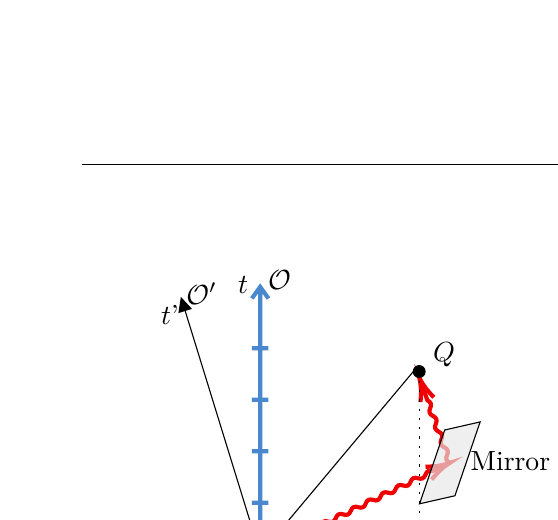
\begin{tikzpicture}[x=0.75pt,y=0.75pt,yscale=-.8,xscale=.8]
	%uncomment if require: \path (0,301); %set diagram left start at 0, and has height of 301
	
	%Straight Lines [id:da9494350226062716] 
	\draw [color={rgb, 255:red, 240; green, 0; blue, 0 }  ,draw opacity=1 ][line width=1.5]    (203.83,183) .. controls (204.6,180.77) and (206.1,180.05) .. (208.33,180.82) .. controls (210.56,181.59) and (212.06,180.87) .. (212.83,178.64) .. controls (213.6,176.41) and (215.1,175.69) .. (217.33,176.47) .. controls (219.56,177.24) and (221.06,176.52) .. (221.83,174.29) .. controls (222.6,172.06) and (224.1,171.34) .. (226.33,172.11) .. controls (228.56,172.88) and (230.06,172.16) .. (230.83,169.93) .. controls (231.6,167.7) and (233.1,166.98) .. (235.33,167.76) .. controls (237.56,168.53) and (239.06,167.81) .. (239.83,165.58) .. controls (240.6,163.35) and (242.1,162.63) .. (244.33,163.4) .. controls (246.56,164.17) and (248.06,163.45) .. (248.84,161.22) .. controls (249.61,158.99) and (251.11,158.27) .. (253.34,159.05) .. controls (255.57,159.82) and (257.07,159.1) .. (257.84,156.87) .. controls (258.61,154.64) and (260.11,153.92) .. (262.34,154.69) .. controls (264.57,155.46) and (266.07,154.74) .. (266.84,152.51) .. controls (267.61,150.28) and (269.11,149.56) .. (271.34,150.33) .. controls (273.57,151.11) and (275.07,150.39) .. (275.84,148.16) .. controls (276.61,145.93) and (278.11,145.21) .. (280.34,145.98) .. controls (282.57,146.75) and (284.07,146.03) .. (284.84,143.8) .. controls (285.61,141.57) and (287.11,140.85) .. (289.34,141.62) .. controls (291.57,142.4) and (293.07,141.68) .. (293.84,139.45) .. controls (294.61,137.22) and (296.11,136.5) .. (298.34,137.27) .. controls (300.57,138.04) and (302.07,137.32) .. (302.85,135.09) .. controls (303.62,132.86) and (305.12,132.14) .. (307.35,132.91) -- (307.6,132.79) -- (314.8,129.31) ;
	\draw [shift={(317.5,128)}, rotate = 514.1800000000001] [color={rgb, 255:red, 240; green, 0; blue, 0 }  ,draw opacity=1 ][line width=1.5]    (14.21,-4.28) .. controls (9.04,-1.82) and (4.3,-0.39) .. (0,0) .. controls (4.3,0.39) and (9.04,1.82) .. (14.21,4.28)   ;
	
	%Straight Lines [id:da7581825810428611] 
	\draw [color={rgb, 255:red, 240; green, 0; blue, 0 }  ,draw opacity=1 ][line width=1.5]    (317.5,128) .. controls (315.37,126.99) and (314.8,125.42) .. (315.81,123.29) .. controls (316.82,121.16) and (316.25,119.59) .. (314.12,118.59) .. controls (311.99,117.58) and (311.43,116.01) .. (312.44,113.88) .. controls (313.45,111.75) and (312.88,110.18) .. (310.75,109.17) .. controls (308.62,108.17) and (308.05,106.6) .. (309.06,104.47) .. controls (310.07,102.34) and (309.5,100.77) .. (307.37,99.76) .. controls (305.24,98.75) and (304.67,97.18) .. (305.68,95.05) .. controls (306.69,92.92) and (306.13,91.36) .. (304,90.35) -- (302.76,86.9) -- (300.06,79.37) ;
	\draw [shift={(299.05,76.55)}, rotate = 430.27] [color={rgb, 255:red, 240; green, 0; blue, 0 }  ,draw opacity=1 ][line width=1.5]    (14.21,-4.28) .. controls (9.04,-1.82) and (4.3,-0.39) .. (0,0) .. controls (4.3,0.39) and (9.04,1.82) .. (14.21,4.28)   ;
	
	%Straight Lines [id:da9007571954817275] 
	\draw [color={rgb, 255:red, 74; green, 144; blue, 226 }  ,draw opacity=1 ][line width=1.5]    (214.5,169) -- (134.25,280.56) (203.6,194.42) -- (193.86,187.42)(187.84,216.34) -- (178.1,209.33)(172.07,238.26) -- (162.33,231.25)(156.31,260.18) -- (146.56,253.17)(140.54,282.1) -- (130.8,275.09) ;
	\draw [shift={(132.5,283)}, rotate = 305.73] [color={rgb, 255:red, 74; green, 144; blue, 226 }  ,draw opacity=1 ][line width=1.5]    (14.21,-6.37) .. controls (9.04,-2.99) and (4.3,-0.87) .. (0,0) .. controls (4.3,0.87) and (9.04,2.99) .. (14.21,6.37)   ;
	
	%Shape: Axis 2D [id:dp17443576451254783] 
	\draw [color={rgb, 255:red, 73; green, 135; blue, 206 }  ,draw opacity=1 ][line width=1.5]  (186,183) -- (392.5,183)(203.28,22) -- (203.28,205) (385.5,178) -- (392.5,183) -- (385.5,188) (198.28,29) -- (203.28,22) -- (208.28,29) (234.28,178) -- (234.28,188)(265.28,178) -- (265.28,188)(296.28,178) -- (296.28,188)(327.28,178) -- (327.28,188)(358.28,178) -- (358.28,188)(198.28,152) -- (208.28,152)(198.28,121) -- (208.28,121)(198.28,90) -- (208.28,90)(198.28,59) -- (208.28,59) ;
	\draw   ;
	%Shape: Circle [id:dp3508886341135449] 
	\draw  [fill={rgb, 255:red, 0; green, 0; blue, 0 }  ,fill opacity=1 ] (200.28,183) .. controls (200.28,181.04) and (201.87,179.45) .. (203.83,179.45) .. controls (205.79,179.45) and (207.37,181.04) .. (207.37,183) .. controls (207.37,184.96) and (205.79,186.55) .. (203.83,186.55) .. controls (201.87,186.55) and (200.28,184.96) .. (200.28,183) -- cycle ;
	%Shape: Circle [id:dp21044900151758394] 
	\draw  [fill={rgb, 255:red, 0; green, 0; blue, 0 }  ,fill opacity=1 ] (295.5,73) .. controls (295.5,71.04) and (297.09,69.45) .. (299.05,69.45) .. controls (301.01,69.45) and (302.59,71.04) .. (302.59,73) .. controls (302.59,74.96) and (301.01,76.55) .. (299.05,76.55) .. controls (297.09,76.55) and (295.5,74.96) .. (295.5,73) -- cycle ;
	%Straight Lines [id:da9075727791620916] 
	\draw    (203.28,183) -- (295.5,73) ;
	
	
	%Straight Lines [id:da5841127763389591] 
	\draw  [dash pattern={on 0.84pt off 2.51pt}]  (299.05,73) -- (299.05,244) ;
	
	
	%Straight Lines [id:da4905999900239695] 
	\draw  [dash pattern={on 4.5pt off 4.5pt}]  (203.83,183) -- (299.05,244) ;
	
	
	%Straight Lines [id:da21567992457799456] 
	\draw    (156.38,30.87) -- (203.28,183) ;
	
	\draw [shift={(155.5,28)}, rotate = 72.87] [fill={rgb, 255:red, 0; green, 0; blue, 0 }  ][line width=0.08]  [draw opacity=0] (8.93,-4.29) -- (0,0) -- (8.93,4.29) -- cycle    ;
	%Shape: Parallelogram [id:dp651969637300376] 
	\draw  [fill={rgb, 255:red, 231; green, 231; blue, 231 }  ,fill opacity=0.67 ] (314.43,108.19) -- (335.74,103.34) -- (320.57,147.81) -- (299.26,152.66) -- cycle ;
	%Shape: Arc [id:dp004235831037150195] 
	\draw  [draw opacity=0] (231.78,168.62) .. controls (235.78,171.9) and (237.86,177.07) .. (236.8,182.57) .. controls (235.48,189.47) and (229.63,194.79) .. (222.69,196.1) -- (220.4,180.73) -- cycle ; \draw   (231.78,168.62) .. controls (235.78,171.9) and (237.86,177.07) .. (236.8,182.57) .. controls (235.48,189.47) and (229.63,194.79) .. (222.69,196.1) ;
	
	% Text Node
	\draw (211,205) node   [align=left] {$\displaystyle \mathcal{P}$};
	% Text Node
	\draw (314,63) node   [align=left] {$\displaystyle Q$};
	% Text Node
	\draw (381,99) node   [align=left] {$ $};
	% Text Node
	\draw (193,21) node   [align=left] {$\displaystyle t$};
	% Text Node
	\draw (405,181) node   [align=left] {$\displaystyle y$};
	% Text Node
	\draw (215,18) node   [align=left] {$\displaystyle \mathcal{O}$};
	% Text Node
	\draw (123,277) node   [align=left] {$\displaystyle x$};
	% Text Node
	\draw (354,127) node   [align=left] {Mirror};
	% Text Node
	\draw (149,39) node   [align=left] {$\displaystyle t$'};
	% Text Node
	\draw (168,26) node   [align=left] {$\displaystyle \mathcal{O} '$};
	% Text Node
	\draw (244,194) node   [align=left] {45$\displaystyle ^{\circ }$};
	\end{tikzpicture}
	\caption{Propagation of a light ray (in red wiggling line) from point P to Q via reflection from a mirror.}
	\label{mirror1}
\end{figure}

Consider now just the $x-y$ projection of this light ray, sketched in Figure~\ref{mirror2}. The angle of incidence to the mirror is $\alpha$, and by the well-known Law of Reflection, the reflection angle is also $\alpha$.

From the diagram, we can easily read off the light ray's total distance traveled in the x-direction as $\Delta x$ and in the y-direction as $h+ (h-\Delta y)$. The time required for the light ray to travel this amount is labeled $\Delta t$, and can be solved for shortly.

\begin{figure}[h!]
	\centering
	\tikzset{every picture/.style={line width=0.75pt}} %set default line width to 0.75pt        
	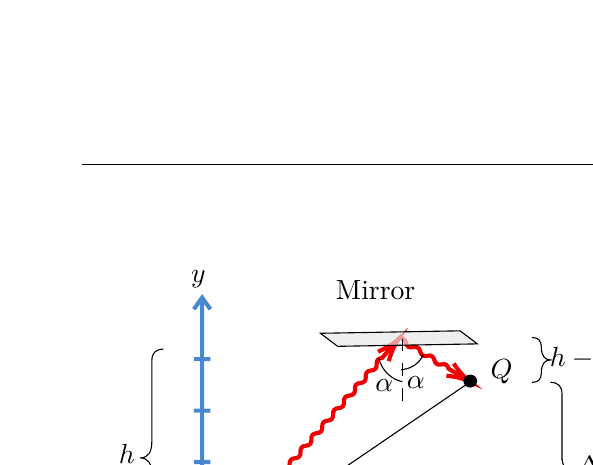
\begin{tikzpicture}[x=0.75pt,y=0.75pt,yscale=-.8,xscale=.8]
	%uncomment if require: \path (0,301); %set diagram left start at 0, and has height of 301
	
	%Straight Lines [id:da36455565985335814] 
	\draw [color={rgb, 255:red, 240; green, 0; blue, 0 }  ,draw opacity=1 ][line width=1.5]    (203.5,182.89) .. controls (203.33,180.54) and (204.43,179.28) .. (206.78,179.11) .. controls (209.13,178.95) and (210.23,177.69) .. (210.06,175.34) .. controls (209.89,172.99) and (210.98,171.73) .. (213.33,171.56) .. controls (215.68,171.4) and (216.78,170.14) .. (216.61,167.79) .. controls (216.44,165.44) and (217.54,164.18) .. (219.89,164.01) .. controls (222.24,163.84) and (223.34,162.58) .. (223.17,160.23) .. controls (223,157.88) and (224.09,156.63) .. (226.44,156.46) .. controls (228.79,156.29) and (229.89,155.03) .. (229.72,152.68) .. controls (229.55,150.33) and (230.65,149.07) .. (233,148.91) .. controls (235.35,148.74) and (236.45,147.48) .. (236.28,145.13) .. controls (236.11,142.78) and (237.21,141.52) .. (239.56,141.36) .. controls (241.91,141.19) and (243,139.93) .. (242.83,137.58) .. controls (242.66,135.23) and (243.76,133.97) .. (246.11,133.8) .. controls (248.46,133.64) and (249.56,132.38) .. (249.39,130.03) .. controls (249.22,127.68) and (250.32,126.42) .. (252.67,126.25) .. controls (255.02,126.08) and (256.11,124.83) .. (255.94,122.48) .. controls (255.77,120.13) and (256.87,118.87) .. (259.22,118.7) .. controls (261.57,118.53) and (262.67,117.27) .. (262.5,114.92) .. controls (262.33,112.57) and (263.43,111.31) .. (265.78,111.15) .. controls (268.13,110.98) and (269.23,109.72) .. (269.06,107.37) .. controls (268.89,105.02) and (269.98,103.77) .. (272.33,103.6) .. controls (274.68,103.43) and (275.78,102.17) .. (275.61,99.82) .. controls (275.44,97.47) and (276.54,96.21) .. (278.89,96.05) .. controls (281.24,95.88) and (282.34,94.62) .. (282.17,92.27) .. controls (282,89.92) and (283.09,88.66) .. (285.44,88.49) .. controls (287.79,88.33) and (288.89,87.07) .. (288.72,84.72) .. controls (288.55,82.37) and (289.65,81.11) .. (292,80.94) .. controls (294.35,80.78) and (295.45,79.52) .. (295.28,77.17) .. controls (295.11,74.82) and (296.2,73.56) .. (298.55,73.39) .. controls (300.9,73.23) and (302,71.97) .. (301.83,69.62) .. controls (301.66,67.27) and (302.76,66.01) .. (305.11,65.84) .. controls (307.46,65.67) and (308.56,64.41) .. (308.39,62.06) .. controls (308.22,59.71) and (309.32,58.45) .. (311.67,58.29) -- (314.57,54.95) -- (319.81,48.9) ;
	\draw [shift={(321.78,46.64)}, rotate = 490.96] [color={rgb, 255:red, 240; green, 0; blue, 0 }  ,draw opacity=1 ][line width=1.5]    (14.21,-4.28) .. controls (9.04,-1.82) and (4.3,-0.39) .. (0,0) .. controls (4.3,0.39) and (9.04,1.82) .. (14.21,4.28)   ;
	
	%Straight Lines [id:da16817630207825296] 
	\draw [color={rgb, 255:red, 240; green, 0; blue, 0 }  ,draw opacity=1 ][line width=1.5]    (321.78,46.64) .. controls (324.07,46.08) and (325.49,46.94) .. (326.05,49.23) .. controls (326.62,51.52) and (328.04,52.38) .. (330.33,51.82) .. controls (332.62,51.26) and (334.04,52.12) .. (334.61,54.41) .. controls (335.17,56.7) and (336.59,57.56) .. (338.88,57) .. controls (341.17,56.44) and (342.59,57.3) .. (343.16,59.59) .. controls (343.73,61.88) and (345.15,62.74) .. (347.44,62.18) .. controls (349.73,61.62) and (351.16,62.49) .. (351.71,64.78) -- (355.36,66.99) -- (362.21,71.13) ;
	\draw [shift={(364.77,72.69)}, rotate = 211.21] [color={rgb, 255:red, 240; green, 0; blue, 0 }  ,draw opacity=1 ][line width=1.5]    (14.21,-4.28) .. controls (9.04,-1.82) and (4.3,-0.39) .. (0,0) .. controls (4.3,0.39) and (9.04,1.82) .. (14.21,4.28)   ;
	
	%Shape: Axis 2D [id:dp6535056270706749] 
	\draw [color={rgb, 255:red, 73; green, 135; blue, 206 }  ,draw opacity=1 ][line width=1.5]  (186,183) -- (392.5,183)(203.28,22) -- (203.28,205) (385.5,178) -- (392.5,183) -- (385.5,188) (198.28,29) -- (203.28,22) -- (208.28,29) (234.28,178) -- (234.28,188)(265.28,178) -- (265.28,188)(296.28,178) -- (296.28,188)(327.28,178) -- (327.28,188)(358.28,178) -- (358.28,188)(198.28,152) -- (208.28,152)(198.28,121) -- (208.28,121)(198.28,90) -- (208.28,90)(198.28,59) -- (208.28,59) ;
	\draw   ;
	%Shape: Circle [id:dp8552343221378937] 
	\draw  [fill={rgb, 255:red, 0; green, 0; blue, 0 }  ,fill opacity=1 ] (200.28,183) .. controls (200.28,181.04) and (201.87,179.45) .. (203.83,179.45) .. controls (205.79,179.45) and (207.37,181.04) .. (207.37,183) .. controls (207.37,184.96) and (205.79,186.55) .. (203.83,186.55) .. controls (201.87,186.55) and (200.28,184.96) .. (200.28,183) -- cycle ;
	%Straight Lines [id:da5063005091976327] 
	\draw    (203.28,182.89) -- (364.77,72.69) ;
	
	
	%Shape: Parallelogram [id:dp978215533235341] 
	\draw  [fill={rgb, 255:red, 231; green, 231; blue, 231 }  ,fill opacity=0.67 ] (284.9,51.31) -- (274.51,43.45) -- (358.65,41.97) -- (369.05,49.83) -- cycle ;
	%Shape: Ellipse [id:dp8465608585817961] 
	\draw  [fill={rgb, 255:red, 0; green, 0; blue, 0 }  ,fill opacity=1 ] (360.98,72.24) .. controls (360.98,70.28) and (362.68,68.69) .. (364.77,68.69) .. controls (366.87,68.69) and (368.56,70.28) .. (368.56,72.24) .. controls (368.56,74.2) and (366.87,75.79) .. (364.77,75.79) .. controls (362.68,75.79) and (360.98,74.2) .. (360.98,72.24) -- cycle ;
	%Straight Lines [id:da7212813545531227] 
	\draw  [dash pattern={on 4.5pt off 4.5pt}]  (323.71,46.64) -- (323.71,86) ;
	
	
	%Shape: Arc [id:dp8732872732226287] 
	\draw  [draw opacity=0] (336.46,56.31) .. controls (335.44,58.72) and (333.74,60.88) .. (331.38,62.53) .. controls (328.92,64.25) and (326.06,65.19) .. (323.13,65.39) -- (320.9,49.77) -- cycle ; \draw   (336.46,56.31) .. controls (335.44,58.72) and (333.74,60.88) .. (331.38,62.53) .. controls (328.92,64.25) and (326.06,65.19) .. (323.13,65.39) ;
	%Shape: Arc [id:dp903029591672244] 
	\draw  [draw opacity=0] (323.87,72.59) .. controls (320.69,71.93) and (317.65,70.38) .. (315.08,67.92) .. controls (312.39,65.34) and (310.55,62.09) .. (309.6,58.58) -- (328.05,52.09) -- cycle ; \draw   (323.87,72.59) .. controls (320.69,71.93) and (317.65,70.38) .. (315.08,67.92) .. controls (312.39,65.34) and (310.55,62.09) .. (309.6,58.58) ;
	%Shape: Brace [id:dp9219084565833189] 
	\draw   (180,53) .. controls (175.33,53) and (173,55.33) .. (173,60) -- (173,108.5) .. controls (173,115.17) and (170.67,118.5) .. (166,118.5) .. controls (170.67,118.5) and (173,121.83) .. (173,128.5)(173,125.5) -- (173,177) .. controls (173,181.67) and (175.33,184) .. (180,184) ;
	%Shape: Brace [id:dp232442639060507] 
	\draw   (204,208) .. controls (204,212.67) and (206.33,215) .. (211,215) -- (273.75,215) .. controls (280.42,215) and (283.75,217.33) .. (283.75,222) .. controls (283.75,217.33) and (287.08,215) .. (293.75,215)(290.75,215) -- (356.5,215) .. controls (361.17,215) and (363.5,212.67) .. (363.5,208) ;
	%Shape: Brace [id:dp49829432158649345] 
	\draw   (413,181) .. controls (417.67,181) and (420,178.67) .. (420,174) -- (420,137) .. controls (420,130.33) and (422.33,127) .. (427,127) .. controls (422.33,127) and (420,123.67) .. (420,117)(420,120) -- (420,80) .. controls (420,75.33) and (417.67,73) .. (413,73) ;
	%Shape: Brace [id:dp9113194227194905] 
	\draw   (402,73) .. controls (405.71,73) and (407.56,71.15) .. (407.56,67.44) -- (407.56,67.44) .. controls (407.56,62.15) and (409.41,59.5) .. (413.12,59.5) .. controls (409.41,59.5) and (407.56,56.85) .. (407.56,51.56)(407.56,53.94) -- (407.56,51.56) .. controls (407.56,47.85) and (405.71,46) .. (402,46) ;
	
	% Text Node
	\draw (211,196) node   [align=left] {$\displaystyle \mathcal{P}$};
	% Text Node
	\draw (383.66,66.67) node   [align=left] {$\displaystyle Q$};
	% Text Node
	\draw (201,11) node   [align=left] {$\displaystyle y$};
	% Text Node
	\draw (405,182) node   [align=left] {$\displaystyle x$};
	% Text Node
	\draw (307.76,17.59) node   [align=left] {Mirror};
	% Text Node
	\draw (313,75.02) node   [align=left] {$\displaystyle \alpha $};
	% Text Node
	\draw (332,73.02) node   [align=left] {$\displaystyle \alpha $};
	% Text Node
	\draw (158,116) node   [align=left] {$\displaystyle h$};
	% Text Node
	\draw (284,235) node   [align=left] {$\displaystyle \Delta x$};
	% Text Node
	\draw (441,125) node   [align=left] {$\displaystyle \Delta y$};
	% Text Node
	\draw (439,59) node   [align=left] {$\displaystyle h-\Delta y$};
	\end{tikzpicture}
	\caption{$x-y$ projection of the light ray's path from Figure~\ref{mirror1}.}
	\label{mirror2}
\end{figure}

Light rays travel along null intervals, and so for the light ray, we can just substitute the distances measured above into the expression for calculating the length of a lightlike separated interval, Equation~\ref{s} with the condition that $\Delta s = 0$:

\beq
\begin{aligned}
& 0 = -(\Delta t)^2 + (\Delta x)^2 + (h+h-\Delta y)^2 \\
& \Rightarrow (\Delta t)^2 = (\Delta x)^2 + (2h - \Delta y)^2
\end{aligned}
\label{lightinterval}
\eeq

This is the time difference between P and Q as measured by $\mathcal{O}$. Equivalently, it is the time required for light to traverse a path from P to Q.

Let us now measure $\Delta s$ in the $\mathcal{O}$ frame. This is done simply by substituting the above expression for the $\Delta t$ into Equation~\ref{s}, along with the measured $\Delta x$ and $\Delta y$:

\beq
\begin{aligned}
	(\Delta s)^2 &= -[(\Delta x)^2 + (2h - \Delta y)^2] + (\Delta x^2) + (\Delta y)^2 \\
	& = (\Delta y)^2 - (2h - \Delta y)^2
\end{aligned}
\label{Ointerval}
\eeq

Note that this interval is timelike, since the right hand side of Equation~\ref{Ointerval} is $<0$.

In a new frame, Figure~\ref{mirror2} would look essentially the same, except with every distance and angle labeled with a prime. There is an additional caveat; the angles $\alpha$ denoting the angles of incidence and reflection when the light ray strikes the mirror may in general be different angles $\alpha_I'$ and $\alpha_R'$.

In order to show that $\Delta s$ is invariant between these two frames, we must prove two lemmas:

\begin{enumerate}
\item $\alpha_I' = \alpha_R'$, i.e. that the Law of Reflection still holds, and
\item $\Delta y' = \Delta y$ and $h' = h$, i.e. that distances perpendicular to the relative velocity $\vec{v}$ of frames $\mathcal{O}$ and $\mathcal{O'}$ do not transform. 	
\end{enumerate}

These are easy to show with simple thought experiments and the strict principle of relativity -- that events which occur in one frame must also occur in all other frames.

\begin{sidebox}[Lemma 1]
Consider two mirrors bouncing light between each other continuously, as in Figure~\ref{mirror3}a. The light moves perpendicular to the mirrors. Each time light strikes a mirror is an event. 

In a new frame moving with respect to the rest frame of the mirrors, the light appears to be bouncing against each mirror at an angle, since the mirrors themselves are apparently moving in this frame. This is shown in Figure~\ref{mirror3}b. In particular, the rays strike a mirror at some angle $\alpha_{I}'$ and are reflected at $\alpha_{R}'$.

If $\alpha_{I}' \neq \alpha_{R}'$, then this implies that the light ray's path is not symmetric up and down. As a consequence, the light ray emitted from the bottom mirror will reflect from the top mirror and strike the bottom mirror again in a different spot than where it was emitted. The result is that the light ray would "drift" off of the mirror slowly in this moving frame, while it does not in the rest frame.

This contradiction is not tolerable; the events seen in one frame must also occur in the other by the principle of relativity. Hence it must be the case that $\alpha{I}' \neq \alpha{R}'$ in all frames, and so the Law of Reflection holds.
\end{sidebox}

\begin{figure}[t!]
	\centering
	\begin{subfigure}[t]{0.45\linewidth}
		\centering
		\tikzset{every picture/.style={line width=0.75pt}} %set default line width to 0.75pt        
		\begin{tikzpicture}[x=0.75pt,y=0.75pt,yscale=-.8,xscale=.8]
		%uncomment if require: \path (0,301); %set diagram left start at 0, and has height of 301
		
		%Straight Lines [id:da24248507832497057] 
		\draw [color={rgb, 255:red, 240; green, 0; blue, 0 }  ,draw opacity=1 ][line width=1.5]    (315.78,153.64) .. controls (314.11,151.97) and (314.11,150.31) .. (315.78,148.64) .. controls (317.45,146.97) and (317.45,145.31) .. (315.78,143.64) .. controls (314.11,141.97) and (314.11,140.31) .. (315.78,138.64) .. controls (317.45,136.97) and (317.45,135.31) .. (315.78,133.64) .. controls (314.11,131.97) and (314.11,130.31) .. (315.78,128.64) .. controls (317.45,126.97) and (317.45,125.31) .. (315.78,123.64) .. controls (314.11,121.97) and (314.11,120.31) .. (315.78,118.64) .. controls (317.45,116.97) and (317.45,115.31) .. (315.78,113.64) .. controls (314.11,111.97) and (314.11,110.31) .. (315.78,108.64) .. controls (317.45,106.97) and (317.45,105.31) .. (315.78,103.64) .. controls (314.11,101.97) and (314.11,100.31) .. (315.78,98.64) .. controls (317.45,96.97) and (317.45,95.31) .. (315.78,93.64) .. controls (314.11,91.97) and (314.11,90.31) .. (315.78,88.64) .. controls (317.45,86.97) and (317.45,85.31) .. (315.78,83.64) .. controls (314.11,81.97) and (314.11,80.31) .. (315.78,78.64) .. controls (317.45,76.97) and (317.45,75.31) .. (315.78,73.64) .. controls (314.11,71.97) and (314.11,70.31) .. (315.78,68.64) .. controls (317.45,66.97) and (317.45,65.31) .. (315.78,63.64) -- (315.78,59.02) -- (315.78,51.02) ;
		\draw [shift={(315.78,48.02)}, rotate = 450] [color={rgb, 255:red, 240; green, 0; blue, 0 }  ,draw opacity=1 ][line width=1.5]    (14.21,-4.28) .. controls (9.04,-1.82) and (4.3,-0.39) .. (0,0) .. controls (4.3,0.39) and (9.04,1.82) .. (14.21,4.28)   ;
		
		%Straight Lines [id:da5664703361793721] 
		\draw [color={rgb, 255:red, 240; green, 0; blue, 0 }  ,draw opacity=1 ][line width=1.5]    (326.78,46.64) .. controls (328.45,48.31) and (328.45,49.97) .. (326.78,51.64) .. controls (325.11,53.31) and (325.11,54.97) .. (326.78,56.64) .. controls (328.45,58.31) and (328.45,59.97) .. (326.78,61.64) .. controls (325.11,63.31) and (325.11,64.97) .. (326.78,66.64) .. controls (328.45,68.31) and (328.45,69.97) .. (326.78,71.64) .. controls (325.11,73.31) and (325.11,74.97) .. (326.78,76.64) .. controls (328.45,78.31) and (328.45,79.97) .. (326.78,81.64) .. controls (325.11,83.31) and (325.11,84.97) .. (326.78,86.64) .. controls (328.45,88.31) and (328.45,89.97) .. (326.78,91.64) .. controls (325.11,93.31) and (325.11,94.97) .. (326.78,96.64) .. controls (328.45,98.31) and (328.45,99.97) .. (326.78,101.64) .. controls (325.11,103.31) and (325.11,104.97) .. (326.78,106.64) .. controls (328.45,108.31) and (328.45,109.97) .. (326.78,111.64) .. controls (325.11,113.31) and (325.11,114.97) .. (326.78,116.64) .. controls (328.45,118.31) and (328.45,119.97) .. (326.78,121.64) .. controls (325.11,123.31) and (325.11,124.97) .. (326.78,126.64) .. controls (328.45,128.31) and (328.45,129.97) .. (326.78,131.64) .. controls (325.11,133.31) and (325.11,134.97) .. (326.78,136.64) .. controls (328.45,138.31) and (328.45,139.97) .. (326.78,141.64) -- (326.78,143.02) -- (326.78,151.02) ;
		\draw [shift={(326.78,154.02)}, rotate = 270] [color={rgb, 255:red, 240; green, 0; blue, 0 }  ,draw opacity=1 ][line width=1.5]    (14.21,-4.28) .. controls (9.04,-1.82) and (4.3,-0.39) .. (0,0) .. controls (4.3,0.39) and (9.04,1.82) .. (14.21,4.28)   ;
		
		%Shape: Parallelogram [id:dp6374544736822019] 
		\draw  [fill={rgb, 255:red, 231; green, 231; blue, 231 }  ,fill opacity=0.67 ] (284.9,51.31) -- (274.51,43.45) -- (358.65,41.97) -- (369.05,49.83) -- cycle ;
		%Shape: Parallelogram [id:dp06929544235754515] 
		\draw  [fill={rgb, 255:red, 231; green, 231; blue, 231 }  ,fill opacity=0.67 ] (281.9,158.31) -- (271.51,150.45) -- (355.65,148.97) -- (366.05,156.83) -- cycle ;
		\end{tikzpicture}
		\caption{Thought experiment bouncing light rays between mirrors.}
	\end{subfigure}
	\qquad
	\begin{subfigure}[t]{0.45\linewidth}
		\centering
		\tikzset{every picture/.style={line width=0.75pt}} %set default line width to 0.75pt        
		\begin{tikzpicture}[x=0.75pt,y=0.75pt,yscale=-.8,xscale=.8]
		%uncomment if require: \path (0,301); %set diagram left start at 0, and has height of 301
		
		%Straight Lines [id:da30853539264163365] 
		\draw [color={rgb, 255:red, 240; green, 0; blue, 0 }  ,draw opacity=1 ][line width=1.5]    (184.78,157.64) .. controls (184.42,155.31) and (185.41,153.96) .. (187.74,153.61) .. controls (190.07,153.25) and (191.05,151.91) .. (190.7,149.58) .. controls (190.34,147.25) and (191.32,145.91) .. (193.65,145.55) .. controls (195.98,145.19) and (196.96,143.85) .. (196.61,141.52) .. controls (196.26,139.19) and (197.24,137.85) .. (199.57,137.49) .. controls (201.9,137.13) and (202.89,135.78) .. (202.53,133.45) .. controls (202.18,131.12) and (203.16,129.78) .. (205.49,129.42) .. controls (207.82,129.06) and (208.8,127.72) .. (208.45,125.39) .. controls (208.09,123.06) and (209.07,121.72) .. (211.4,121.36) .. controls (213.73,121) and (214.71,119.66) .. (214.36,117.33) .. controls (214.01,115) and (214.99,113.66) .. (217.32,113.3) .. controls (219.65,112.94) and (220.63,111.6) .. (220.28,109.27) .. controls (219.93,106.94) and (220.91,105.6) .. (223.24,105.24) .. controls (225.57,104.88) and (226.55,103.54) .. (226.2,101.21) .. controls (225.84,98.88) and (226.82,97.54) .. (229.15,97.18) .. controls (231.48,96.82) and (232.46,95.48) .. (232.11,93.15) .. controls (231.76,90.82) and (232.74,89.48) .. (235.07,89.12) .. controls (237.4,88.76) and (238.39,87.41) .. (238.03,85.08) .. controls (237.68,82.75) and (238.66,81.41) .. (240.99,81.05) .. controls (243.32,80.69) and (244.3,79.35) .. (243.95,77.02) .. controls (243.6,74.69) and (244.58,73.35) .. (246.91,72.99) .. controls (249.24,72.63) and (250.22,71.29) .. (249.86,68.96) .. controls (249.51,66.63) and (250.49,65.29) .. (252.82,64.93) .. controls (255.15,64.57) and (256.13,63.23) .. (255.78,60.9) -- (258.27,57.51) -- (263,51.06) ;
		\draw [shift={(264.78,48.64)}, rotate = 486.28] [color={rgb, 255:red, 240; green, 0; blue, 0 }  ,draw opacity=1 ][line width=1.5]    (14.21,-4.28) .. controls (9.04,-1.82) and (4.3,-0.39) .. (0,0) .. controls (4.3,0.39) and (9.04,1.82) .. (14.21,4.28)   ;
		
		%Straight Lines [id:da651790824445525] 
		\draw [color={rgb, 255:red, 240; green, 0; blue, 0 }  ,draw opacity=1 ][line width=1.5]    (264.78,48.64) .. controls (267.12,48.89) and (268.16,50.19) .. (267.91,52.54) .. controls (267.66,54.89) and (268.7,56.18) .. (271.05,56.43) .. controls (273.39,56.69) and (274.43,57.99) .. (274.18,60.33) .. controls (273.93,62.68) and (274.97,63.97) .. (277.32,64.22) .. controls (279.66,64.48) and (280.7,65.78) .. (280.45,68.12) .. controls (280.2,70.46) and (281.24,71.76) .. (283.58,72.01) .. controls (285.93,72.26) and (286.97,73.56) .. (286.72,75.91) .. controls (286.47,78.25) and (287.51,79.55) .. (289.85,79.8) .. controls (292.2,80.05) and (293.24,81.35) .. (292.99,83.7) .. controls (292.74,86.04) and (293.78,87.34) .. (296.12,87.6) .. controls (298.47,87.85) and (299.51,89.14) .. (299.26,91.49) .. controls (299.01,93.83) and (300.05,95.13) .. (302.39,95.39) .. controls (304.73,95.64) and (305.77,96.94) .. (305.52,99.28) .. controls (305.27,101.63) and (306.31,102.93) .. (308.66,103.18) .. controls (311,103.43) and (312.04,104.73) .. (311.79,107.07) .. controls (311.54,109.42) and (312.58,110.72) .. (314.93,110.97) .. controls (317.27,111.23) and (318.31,112.53) .. (318.06,114.87) .. controls (317.81,117.22) and (318.85,118.51) .. (321.2,118.76) .. controls (323.54,119.02) and (324.58,120.32) .. (324.33,122.66) .. controls (324.08,125) and (325.12,126.3) .. (327.46,126.55) .. controls (329.81,126.8) and (330.85,128.1) .. (330.6,130.45) .. controls (330.35,132.79) and (331.39,134.09) .. (333.73,134.34) .. controls (336.08,134.59) and (337.12,135.89) .. (336.87,138.24) .. controls (336.62,140.58) and (337.66,141.88) .. (340,142.14) .. controls (342.35,142.39) and (343.39,143.68) .. (343.14,146.03) -- (345.88,149.45) -- (350.9,155.68) ;
		\draw [shift={(352.78,158.02)}, rotate = 231.18] [color={rgb, 255:red, 240; green, 0; blue, 0 }  ,draw opacity=1 ][line width=1.5]    (14.21,-4.28) .. controls (9.04,-1.82) and (4.3,-0.39) .. (0,0) .. controls (4.3,0.39) and (9.04,1.82) .. (14.21,4.28)   ;
		
		%Shape: Parallelogram [id:dp35373648380097755] 
		\draw  [fill={rgb, 255:red, 231; green, 231; blue, 231 }  ,fill opacity=0.67 ] (227.9,53.31) -- (217.51,45.45) -- (301.65,43.97) -- (312.05,51.83) -- cycle ;
		%Shape: Parallelogram [id:dp723902019214397] 
		\draw  [fill={rgb, 255:red, 231; green, 231; blue, 231 }  ,fill opacity=0.67 ] (147.9,162.31) -- (137.51,154.45) -- (221.65,152.97) -- (232.05,160.83) -- cycle ;
		%Shape: Parallelogram [id:dp579143474020132] 
		\draw  [fill={rgb, 255:red, 231; green, 231; blue, 231 }  ,fill opacity=0.67 ] (317.9,161.69) -- (307.51,153.82) -- (391.65,152.34) -- (402.05,160.21) -- cycle ;
		%Shape: Parallelogram [id:dp7762198970376433] 
		\draw  [fill={rgb, 255:red, 231; green, 231; blue, 231 }  ,fill opacity=0.67 ] (393.9,53.31) -- (383.51,45.45) -- (467.65,43.97) -- (478.05,51.83) -- cycle ;
		%Straight Lines [id:da1892052709651828] 
		\draw [color={rgb, 255:red, 240; green, 0; blue, 0 }  ,draw opacity=1 ][line width=1.5]    (350.78,157.64) .. controls (350.42,155.31) and (351.41,153.96) .. (353.74,153.61) .. controls (356.07,153.25) and (357.05,151.91) .. (356.7,149.58) .. controls (356.34,147.25) and (357.32,145.91) .. (359.65,145.55) .. controls (361.98,145.19) and (362.96,143.85) .. (362.61,141.52) .. controls (362.26,139.19) and (363.24,137.85) .. (365.57,137.49) .. controls (367.9,137.13) and (368.89,135.78) .. (368.53,133.45) .. controls (368.18,131.12) and (369.16,129.78) .. (371.49,129.42) .. controls (373.82,129.06) and (374.8,127.72) .. (374.45,125.39) .. controls (374.09,123.06) and (375.07,121.72) .. (377.4,121.36) .. controls (379.73,121) and (380.71,119.66) .. (380.36,117.33) .. controls (380.01,115) and (380.99,113.66) .. (383.32,113.3) .. controls (385.65,112.94) and (386.63,111.6) .. (386.28,109.27) .. controls (385.93,106.94) and (386.91,105.6) .. (389.24,105.24) .. controls (391.57,104.88) and (392.55,103.54) .. (392.2,101.21) .. controls (391.84,98.88) and (392.82,97.54) .. (395.15,97.18) .. controls (397.48,96.82) and (398.46,95.48) .. (398.11,93.15) .. controls (397.76,90.82) and (398.74,89.48) .. (401.07,89.12) .. controls (403.4,88.76) and (404.39,87.41) .. (404.03,85.08) .. controls (403.68,82.75) and (404.66,81.41) .. (406.99,81.05) .. controls (409.32,80.69) and (410.3,79.35) .. (409.95,77.02) .. controls (409.6,74.69) and (410.58,73.35) .. (412.91,72.99) .. controls (415.24,72.63) and (416.22,71.29) .. (415.86,68.96) .. controls (415.51,66.63) and (416.49,65.29) .. (418.82,64.93) .. controls (421.15,64.57) and (422.13,63.23) .. (421.78,60.9) -- (424.27,57.51) -- (429,51.06) ;
		\draw [shift={(430.78,48.64)}, rotate = 486.28] [color={rgb, 255:red, 240; green, 0; blue, 0 }  ,draw opacity=1 ][line width=1.5]    (14.21,-4.28) .. controls (9.04,-1.82) and (4.3,-0.39) .. (0,0) .. controls (4.3,0.39) and (9.04,1.82) .. (14.21,4.28)   ;
		
		%Straight Lines [id:da7759457471770823] 
		\draw  [dash pattern={on 4.5pt off 4.5pt}]  (264.78,48.64) -- (264.78,101.02) ;
		
		
		%Shape: Arc [id:dp9668414920314963] 
		\draw  [draw opacity=0] (265.98,80.91) .. controls (262.76,80.58) and (259.58,79.35) .. (256.77,77.16) .. controls (253.82,74.87) and (251.67,71.83) .. (250.36,68.43) -- (268.05,60.09) -- cycle ; \draw   (265.98,80.91) .. controls (262.76,80.58) and (259.58,79.35) .. (256.77,77.16) .. controls (253.82,74.87) and (251.67,71.83) .. (250.36,68.43) ;
		%Shape: Arc [id:dp32971833998280875] 
		\draw  [draw opacity=0] (287.1,78.29) .. controls (284.78,81.74) and (281.48,84.61) .. (277.31,86.48) .. controls (272.94,88.44) and (268.2,89.05) .. (263.57,88.49) -- (264.75,63.44) -- cycle ; \draw   (287.1,78.29) .. controls (284.78,81.74) and (281.48,84.61) .. (277.31,86.48) .. controls (272.94,88.44) and (268.2,89.05) .. (263.57,88.49) ;
		
		% Text Node
		\draw (253,90) node   [align=left] {$\displaystyle \alpha _{I} '$};
		% Text Node
		\draw (281,93) node   [align=left] {$\displaystyle \alpha _{R} '$};
		\end{tikzpicture}
		\caption{The same experiment as in Figure~\ref{mirror3}a, but in a moving frame.}
	\end{subfigure}
	\caption{}
	\label{mirror3}
\end{figure}

\begin{sidebox}[Lemma 2]

Consider an experiment where two hollow tubes of precisely the same radius are exactly aligned horizontally along their central axes. These tubes move toward each other and collide at the exact same velocity, as in Figure~\ref{cyl}. The collision is an event which happens, so all observers must see it at some location in time and space.

	First, as an aside, by cylindrical symmetry of both the tubes and the relative velocity vector $\vec{v}$ between the two frames, any transformation to distances which happen in directions perpendicular to $\vec{v}$ must by cylindrically symmetric as well. In other words, no perpendicular directions to $\vec{v}$ are "preferred" to change in a special way relative to the others.

In the rest frame of one of the cylinders, we may in general observe the other cylinder to have a different shape. Suppose that this second cylinder stretched perpendicularly to the relative velocity of the cylinders, i.e. that the other cylinder expands or shrinks, so that the cylinder's radii has changed.

In this case, the two cylinder now have different radii. This means that their rims will not collide when the cylinders move toward each other. However, this means different events are occurring in different frames, which clearly violates the principle of relativity. 

Consequently, the radii of the cylinders may not change between such a relativistic transformation, and all distances perpendicular to the relative velocity of two frames are preserved in transforming from one of the frames to the other.

\end{sidebox}

\begin{figure}[h]
	\centering
	\begin{subfigure}[t]{0.45\linewidth}
		\centering
		\tikzset{every picture/.style={line width=0.75pt}} %set default line width to 0.75pt        
		\begin{tikzpicture}[x=0.75pt,y=0.75pt,yscale=-.8,xscale=.8]
		%uncomment if require: \path (0,301); %set diagram left start at 0, and has height of 301
		
		%Shape: Can [id:dp12353151642329996] 
		\draw   (141,138) -- (89,138) .. controls (84.03,138) and (80,124.57) .. (80,108) .. controls (80,91.43) and (84.03,78) .. (89,78) -- (141,78) .. controls (145.97,78) and (150,91.43) .. (150,108) .. controls (150,124.57) and (145.97,138) .. (141,138) .. controls (136.03,138) and (132,124.57) .. (132,108) .. controls (132,91.43) and (136.03,78) .. (141,78) ;
		%Shape: Can [id:dp8700266421811906] 
		\draw   (336,138) -- (284,138) .. controls (279.03,138) and (275,124.57) .. (275,108) .. controls (275,91.43) and (279.03,78) .. (284,78) -- (336,78) .. controls (340.97,78) and (345,91.43) .. (345,108) .. controls (345,124.57) and (340.97,138) .. (336,138) .. controls (331.03,138) and (327,124.57) .. (327,108) .. controls (327,91.43) and (331.03,78) .. (336,78) ;
		%Straight Lines [id:da6741344517921886] 
		\draw    (141,111) -- (180.5,111) ;
		\draw [shift={(182.5,111)}, rotate = 180] [color={rgb, 255:red, 0; green, 0; blue, 0 }  ][line width=0.75]    (10.93,-3.29) .. controls (6.95,-1.4) and (3.31,-0.3) .. (0,0) .. controls (3.31,0.3) and (6.95,1.4) .. (10.93,3.29)   ;
		
		%Straight Lines [id:da3744733231893391] 
		\draw    (238,111) -- (275,111) ;
		
		\draw [shift={(236,111)}, rotate = 0] [color={rgb, 255:red, 0; green, 0; blue, 0 }  ][line width=0.75]    (10.93,-4.9) .. controls (6.95,-2.3) and (3.31,-0.67) .. (0,0) .. controls (3.31,0.67) and (6.95,2.3) .. (10.93,4.9);
		\end{tikzpicture}
		\caption{Two identical hollow tubes exactly in alignment and moving toward each other, so that they collide when the rims of the tubes touch.}
	\end{subfigure}
	\qquad
	\begin{subfigure}[t]{0.45\linewidth}
		\centering
		\tikzset{every picture/.style={line width=0.75pt}} %set default line width to 0.75pt        
		\begin{tikzpicture}[x=0.75pt,y=0.75pt,yscale=-.8,xscale=.8]
		%uncomment if require: \path (0,301); %set diagram left start at 0, and has height of 301
		
		%Shape: Can [id:dp7569599162808271] 
		\draw   (141,138) -- (89,138) .. controls (84.03,138) and (80,124.57) .. (80,108) .. controls (80,91.43) and (84.03,78) .. (89,78) -- (141,78) .. controls (145.97,78) and (150,91.43) .. (150,108) .. controls (150,124.57) and (145.97,138) .. (141,138) .. controls (136.03,138) and (132,124.57) .. (132,108) .. controls (132,91.43) and (136.03,78) .. (141,78) ;
		%Shape: Can [id:dp16420703944467996] 
		\draw   (305.48,128) -- (279.5,128) .. controls (277.01,128) and (275,121.29) .. (275,113.01) .. controls (275,104.73) and (277.01,98.02) .. (279.5,98.02) -- (305.48,98.02) .. controls (307.97,98.02) and (309.98,104.73) .. (309.98,113.01) .. controls (309.98,121.29) and (307.97,128) .. (305.48,128) .. controls (303,128) and (300.99,121.29) .. (300.99,113.01) .. controls (300.99,104.73) and (303,98.02) .. (305.48,98.02) ;
		%Straight Lines [id:da3996944750743705] 
		\draw    (197.5,111) -- (275,111) ;
		
		\draw [shift={(195.5,111)}, rotate = 0] [color={rgb, 255:red, 0; green, 0; blue, 0 }  ][line width=0.75]    (10.93,-4.9) .. controls (6.95,-2.3) and (3.31,-0.67) .. (0,0) .. controls (3.31,0.67) and (6.95,2.3) .. (10.93,4.9)   ;
		\end{tikzpicture}
		\caption{The same experiment as in Figure~\ref{mirror3} in the frame of the left cylinder, but assuming that the radii of the cylinders may change in different frames.}
	\end{subfigure}
	\caption{}
	\label{cyl}
\end{figure}

With these lemmas proven, we can return to the problem at hand, finding the spacetime interval $\Delta s$ between two events P and Q. 

The lemmas we proved indicate that the analogous diagram to Figure~\ref{mirror2} is identical, with where we need to only replace $\Delta x$ with $\Delta x'$ and $\alpha$ with $\alpha'$; $h$ and $\Delta y$ do not transform.

The spatial and and time intervals between P and Q measured in the $\mathcal{O'}$ frame are given by $(\Delta x')^2, (\Delta y')^2, (\Delta t')^2$. However, in this frame, we can perform the same light-beam experiment shown in Figures~\ref{mirror1} and~\ref{mirror2} to measure what the apparent elapsed time $\Delta t'$ is between events P and Q. Since the diagrams are analogous, the result will also be precisely analogous to Equation~\ref{lightinterval}:

\beq
(\Delta t')^2 = (\Delta x')^2 + (2h - \Delta y)^2
\label{lightinterval2}
\eeq

As a result, the space-time interval between these events calculated in the $\mathcal{O'}$ frame is calculated the same way as in the $\mathcal{O}$ frame:

\beq
\Rightarrow \Rightarrow (\Delta s')^2 = (\Delta y)^2 - (2h - \Delta y)^2 = (\Delta s)^2
\label{deltas2}
\eeq

For this reason, $\Delta s$ is often called the "invariant distance" between events.

\section{Relativistic Transformations of Coordinate Systems}

We can be slightly more precise about what we mean by "coordinate system" in the earlier discussions by introducing the idea of the "light clock."

Imagine a regular lattice of several clocks through which we regularly shine beams of light from one to the other to synchronize the clocks appropriately. The ticks of these clocks then denote tick marks along a "time axis," forming a 4-dimensional lattice of coordinates in space and time. An example of such a coordinate system is shown in Figure~\ref{clocks}.

%This next picture will knock your clocks off.
\begin{figure}[]
	\centering
	\tikzset{every picture/.style={line width=0.75pt}} %set default line width to 0.75pt        
	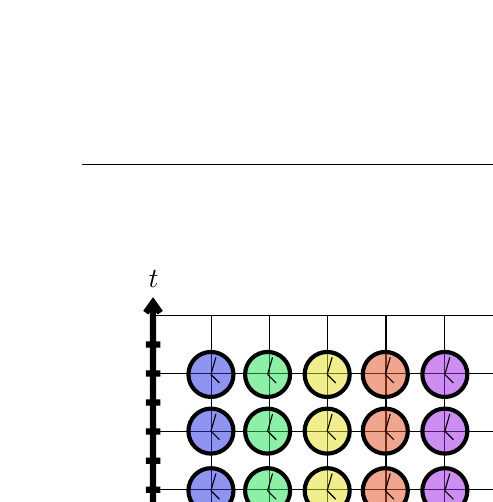
\begin{tikzpicture}[x=0.75pt,y=0.75pt,yscale=-.7,xscale=.7]
	%uncomment if require: \path (0,316.015625); %set diagram left start at 0, and has height of 316.015625
	
	%Shape: Axis 2D [id:dp8320298567254818] 
	\draw [line width=2.25]  (52,278.85) -- (328.5,278.85)(79.65,30) -- (79.65,306.5) (321.5,273.85) -- (328.5,278.85) -- (321.5,283.85) (74.65,37) -- (79.65,30) -- (84.65,37) (99.65,273.85) -- (99.65,283.85)(119.65,273.85) -- (119.65,283.85)(139.65,273.85) -- (139.65,283.85)(159.65,273.85) -- (159.65,283.85)(179.65,273.85) -- (179.65,283.85)(199.65,273.85) -- (199.65,283.85)(219.65,273.85) -- (219.65,283.85)(239.65,273.85) -- (239.65,283.85)(259.65,273.85) -- (259.65,283.85)(279.65,273.85) -- (279.65,283.85)(299.65,273.85) -- (299.65,283.85)(59.65,273.85) -- (59.65,283.85)(74.65,258.85) -- (84.65,258.85)(74.65,238.85) -- (84.65,238.85)(74.65,218.85) -- (84.65,218.85)(74.65,198.85) -- (84.65,198.85)(74.65,178.85) -- (84.65,178.85)(74.65,158.85) -- (84.65,158.85)(74.65,138.85) -- (84.65,138.85)(74.65,118.85) -- (84.65,118.85)(74.65,98.85) -- (84.65,98.85)(74.65,78.85) -- (84.65,78.85)(74.65,58.85) -- (84.65,58.85)(74.65,298.85) -- (84.65,298.85) ;
	\draw   ;
	%Shape: Grid [id:dp7052936952182616] 
	\draw  [draw opacity=0] (80,39) -- (320.5,39) -- (320.5,278.02) -- (80,278.02) -- cycle ; \draw   (80,39) -- (80,278.02)(120,39) -- (120,278.02)(160,39) -- (160,278.02)(200,39) -- (200,278.02)(240,39) -- (240,278.02)(280,39) -- (280,278.02)(320,39) -- (320,278.02) ; \draw   (80,39) -- (320.5,39)(80,79) -- (320.5,79)(80,119) -- (320.5,119)(80,159) -- (320.5,159)(80,199) -- (320.5,199)(80,239) -- (320.5,239) ; \draw    ;
	%Shape: Circle [id:dp38734123820868094] 
	\draw  [fill={rgb, 255:red, 38; green, 49; blue, 226 }  ,fill opacity=0.52 ][line width=1.5]  (104.02,239.51) .. controls (104.02,230.95) and (110.95,224.02) .. (119.51,224.02) .. controls (128.06,224.02) and (135,230.95) .. (135,239.51) .. controls (135,248.06) and (128.06,255) .. (119.51,255) .. controls (110.95,255) and (104.02,248.06) .. (104.02,239.51) -- cycle ;
	%Straight Lines [id:da3732415907025304] 
	\draw    (119.51,239.51) -- (125.39,245.39) ;
	
	
	%Straight Lines [id:da17723096254318582] 
	\draw    (119.51,239.51) -- (122.92,227.74) ;
	
	
	
	%Shape: Circle [id:dp873232004038208] 
	\draw  [fill={rgb, 255:red, 38; green, 49; blue, 226 }  ,fill opacity=0.52 ][line width=1.5]  (104.02,199.51) .. controls (104.02,190.95) and (110.95,184.02) .. (119.51,184.02) .. controls (128.06,184.02) and (135,190.95) .. (135,199.51) .. controls (135,208.06) and (128.06,215) .. (119.51,215) .. controls (110.95,215) and (104.02,208.06) .. (104.02,199.51) -- cycle ;
	%Straight Lines [id:da7618067591473634] 
	\draw    (119.51,199.51) -- (125.39,205.39) ;
	
	
	%Straight Lines [id:da141757157056144] 
	\draw    (119.51,199.51) -- (122.92,187.74) ;
	
	
	
	%Shape: Circle [id:dp8675033778358052] 
	\draw  [fill={rgb, 255:red, 38; green, 49; blue, 226 }  ,fill opacity=0.52 ][line width=1.5]  (104.02,159.51) .. controls (104.02,150.95) and (110.95,144.02) .. (119.51,144.02) .. controls (128.06,144.02) and (135,150.95) .. (135,159.51) .. controls (135,168.06) and (128.06,175) .. (119.51,175) .. controls (110.95,175) and (104.02,168.06) .. (104.02,159.51) -- cycle ;
	%Straight Lines [id:da9804659465251155] 
	\draw    (119.51,159.51) -- (125.39,165.39) ;
	
	
	%Straight Lines [id:da5452434641745356] 
	\draw    (119.51,159.51) -- (122.92,147.74) ;
	
	
	
	%Shape: Circle [id:dp9721469925645583] 
	\draw  [fill={rgb, 255:red, 38; green, 49; blue, 226 }  ,fill opacity=0.52 ][line width=1.5]  (104.02,118.51) .. controls (104.02,109.95) and (110.95,103.02) .. (119.51,103.02) .. controls (128.06,103.02) and (135,109.95) .. (135,118.51) .. controls (135,127.06) and (128.06,134) .. (119.51,134) .. controls (110.95,134) and (104.02,127.06) .. (104.02,118.51) -- cycle ;
	%Straight Lines [id:da6970543195572318] 
	\draw    (119.51,118.51) -- (125.39,124.39) ;
	
	
	%Straight Lines [id:da6768314714271062] 
	\draw    (119.51,118.51) -- (122.92,106.74) ;
	
	
	
	%Shape: Circle [id:dp039174000093122885] 
	\draw  [fill={rgb, 255:red, 38; green, 49; blue, 226 }  ,fill opacity=0.52 ][line width=1.5]  (104.02,79.51) .. controls (104.02,70.95) and (110.95,64.02) .. (119.51,64.02) .. controls (128.06,64.02) and (135,70.95) .. (135,79.51) .. controls (135,88.06) and (128.06,95) .. (119.51,95) .. controls (110.95,95) and (104.02,88.06) .. (104.02,79.51) -- cycle ;
	%Straight Lines [id:da11687388360325834] 
	\draw    (119.51,79.51) -- (125.39,85.39) ;
	
	
	%Straight Lines [id:da8423448504470252] 
	\draw    (119.51,79.51) -- (122.92,67.74) ;
	
	
	
	%Shape: Circle [id:dp8349016851012061] 
	\draw  [fill={rgb, 255:red, 38; green, 226; blue, 88 }  ,fill opacity=0.52 ][line width=1.5]  (143.02,239.51) .. controls (143.02,230.95) and (149.95,224.02) .. (158.51,224.02) .. controls (167.06,224.02) and (174,230.95) .. (174,239.51) .. controls (174,248.06) and (167.06,255) .. (158.51,255) .. controls (149.95,255) and (143.02,248.06) .. (143.02,239.51) -- cycle ;
	%Straight Lines [id:da6621681195035165] 
	\draw [fill={rgb, 255:red, 38; green, 226; blue, 88 }  ,fill opacity=0.52 ]   (158.51,239.51) -- (164.39,245.39) ;
	
	
	%Straight Lines [id:da7898027552573206] 
	\draw [fill={rgb, 255:red, 38; green, 226; blue, 88 }  ,fill opacity=0.52 ]   (158.51,239.51) -- (161.92,227.74) ;
	
	
	
	%Shape: Circle [id:dp10884946662111705] 
	\draw  [fill={rgb, 255:red, 38; green, 226; blue, 88 }  ,fill opacity=0.52 ][line width=1.5]  (143.02,199.51) .. controls (143.02,190.95) and (149.95,184.02) .. (158.51,184.02) .. controls (167.06,184.02) and (174,190.95) .. (174,199.51) .. controls (174,208.06) and (167.06,215) .. (158.51,215) .. controls (149.95,215) and (143.02,208.06) .. (143.02,199.51) -- cycle ;
	%Straight Lines [id:da10152117274299166] 
	\draw [fill={rgb, 255:red, 38; green, 226; blue, 88 }  ,fill opacity=0.52 ]   (158.51,199.51) -- (164.39,205.39) ;
	
	
	%Straight Lines [id:da3365345392519721] 
	\draw [fill={rgb, 255:red, 38; green, 226; blue, 88 }  ,fill opacity=0.52 ]   (158.51,199.51) -- (161.92,187.74) ;
	
	
	
	%Shape: Circle [id:dp4393360754347859] 
	\draw  [fill={rgb, 255:red, 38; green, 226; blue, 88 }  ,fill opacity=0.52 ][line width=1.5]  (143.02,159.51) .. controls (143.02,150.95) and (149.95,144.02) .. (158.51,144.02) .. controls (167.06,144.02) and (174,150.95) .. (174,159.51) .. controls (174,168.06) and (167.06,175) .. (158.51,175) .. controls (149.95,175) and (143.02,168.06) .. (143.02,159.51) -- cycle ;
	%Straight Lines [id:da3012692959779113] 
	\draw [fill={rgb, 255:red, 38; green, 226; blue, 88 }  ,fill opacity=0.52 ]   (158.51,159.51) -- (164.39,165.39) ;
	
	
	%Straight Lines [id:da652471733482952] 
	\draw [fill={rgb, 255:red, 38; green, 226; blue, 88 }  ,fill opacity=0.52 ]   (158.51,159.51) -- (161.92,147.74) ;
	
	
	
	%Shape: Circle [id:dp46520116100665954] 
	\draw  [fill={rgb, 255:red, 38; green, 226; blue, 88 }  ,fill opacity=0.52 ][line width=1.5]  (143.02,118.51) .. controls (143.02,109.95) and (149.95,103.02) .. (158.51,103.02) .. controls (167.06,103.02) and (174,109.95) .. (174,118.51) .. controls (174,127.06) and (167.06,134) .. (158.51,134) .. controls (149.95,134) and (143.02,127.06) .. (143.02,118.51) -- cycle ;
	%Straight Lines [id:da8062709901225151] 
	\draw [fill={rgb, 255:red, 38; green, 226; blue, 88 }  ,fill opacity=0.52 ]   (158.51,118.51) -- (164.39,124.39) ;
	
	
	%Straight Lines [id:da0667928049399722] 
	\draw [fill={rgb, 255:red, 38; green, 226; blue, 88 }  ,fill opacity=0.52 ]   (158.51,118.51) -- (161.92,106.74) ;
	
	
	
	%Shape: Circle [id:dp7323864705001355] 
	\draw  [fill={rgb, 255:red, 38; green, 226; blue, 88 }  ,fill opacity=0.52 ][line width=1.5]  (143.02,79.51) .. controls (143.02,70.95) and (149.95,64.02) .. (158.51,64.02) .. controls (167.06,64.02) and (174,70.95) .. (174,79.51) .. controls (174,88.06) and (167.06,95) .. (158.51,95) .. controls (149.95,95) and (143.02,88.06) .. (143.02,79.51) -- cycle ;
	%Straight Lines [id:da1758849907010962] 
	\draw [fill={rgb, 255:red, 38; green, 226; blue, 88 }  ,fill opacity=0.52 ]   (158.51,79.51) -- (164.39,85.39) ;
	
	
	%Straight Lines [id:da1475934627006137] 
	\draw [fill={rgb, 255:red, 38; green, 226; blue, 88 }  ,fill opacity=0.52 ]   (158.51,79.51) -- (161.92,67.74) ;
	
	
	
	%Shape: Circle [id:dp2973304779282464] 
	\draw  [fill={rgb, 255:red, 226; green, 222; blue, 38 }  ,fill opacity=0.52 ][line width=1.5]  (184.02,239.51) .. controls (184.02,230.95) and (190.95,224.02) .. (199.51,224.02) .. controls (208.06,224.02) and (215,230.95) .. (215,239.51) .. controls (215,248.06) and (208.06,255) .. (199.51,255) .. controls (190.95,255) and (184.02,248.06) .. (184.02,239.51) -- cycle ;
	%Straight Lines [id:da8317754653147911] 
	\draw [fill={rgb, 255:red, 226; green, 222; blue, 38 }  ,fill opacity=0.52 ]   (199.51,239.51) -- (205.39,245.39) ;
	
	
	%Straight Lines [id:da6533894835558924] 
	\draw [fill={rgb, 255:red, 226; green, 222; blue, 38 }  ,fill opacity=0.52 ]   (199.51,239.51) -- (202.92,227.74) ;
	
	
	
	%Shape: Circle [id:dp2728648400916611] 
	\draw  [fill={rgb, 255:red, 226; green, 222; blue, 38 }  ,fill opacity=0.52 ][line width=1.5]  (184.02,199.51) .. controls (184.02,190.95) and (190.95,184.02) .. (199.51,184.02) .. controls (208.06,184.02) and (215,190.95) .. (215,199.51) .. controls (215,208.06) and (208.06,215) .. (199.51,215) .. controls (190.95,215) and (184.02,208.06) .. (184.02,199.51) -- cycle ;
	%Straight Lines [id:da8968791276768493] 
	\draw [fill={rgb, 255:red, 226; green, 222; blue, 38 }  ,fill opacity=0.52 ]   (199.51,199.51) -- (205.39,205.39) ;
	
	
	%Straight Lines [id:da25953374905517523] 
	\draw [fill={rgb, 255:red, 226; green, 222; blue, 38 }  ,fill opacity=0.52 ]   (199.51,199.51) -- (202.92,187.74) ;
	
	
	
	%Shape: Circle [id:dp9112029788049025] 
	\draw  [fill={rgb, 255:red, 226; green, 222; blue, 38 }  ,fill opacity=0.52 ][line width=1.5]  (184.02,159.51) .. controls (184.02,150.95) and (190.95,144.02) .. (199.51,144.02) .. controls (208.06,144.02) and (215,150.95) .. (215,159.51) .. controls (215,168.06) and (208.06,175) .. (199.51,175) .. controls (190.95,175) and (184.02,168.06) .. (184.02,159.51) -- cycle ;
	%Straight Lines [id:da33590920557155113] 
	\draw [fill={rgb, 255:red, 226; green, 222; blue, 38 }  ,fill opacity=0.52 ]   (199.51,159.51) -- (205.39,165.39) ;
	
	
	%Straight Lines [id:da018757906028804783] 
	\draw [fill={rgb, 255:red, 226; green, 222; blue, 38 }  ,fill opacity=0.52 ]   (199.51,159.51) -- (202.92,147.74) ;
	
	
	
	%Shape: Circle [id:dp8444932967751029] 
	\draw  [fill={rgb, 255:red, 226; green, 222; blue, 38 }  ,fill opacity=0.52 ][line width=1.5]  (184.02,118.51) .. controls (184.02,109.95) and (190.95,103.02) .. (199.51,103.02) .. controls (208.06,103.02) and (215,109.95) .. (215,118.51) .. controls (215,127.06) and (208.06,134) .. (199.51,134) .. controls (190.95,134) and (184.02,127.06) .. (184.02,118.51) -- cycle ;
	%Straight Lines [id:da8972976025324482] 
	\draw [fill={rgb, 255:red, 226; green, 222; blue, 38 }  ,fill opacity=0.52 ]   (199.51,118.51) -- (205.39,124.39) ;
	
	
	%Straight Lines [id:da4366407777457908] 
	\draw [fill={rgb, 255:red, 226; green, 222; blue, 38 }  ,fill opacity=0.52 ]   (199.51,118.51) -- (202.92,106.74) ;
	
	
	
	%Shape: Circle [id:dp1573888010003901] 
	\draw  [fill={rgb, 255:red, 226; green, 222; blue, 38 }  ,fill opacity=0.52 ][line width=1.5]  (184.02,79.51) .. controls (184.02,70.95) and (190.95,64.02) .. (199.51,64.02) .. controls (208.06,64.02) and (215,70.95) .. (215,79.51) .. controls (215,88.06) and (208.06,95) .. (199.51,95) .. controls (190.95,95) and (184.02,88.06) .. (184.02,79.51) -- cycle ;
	%Straight Lines [id:da1745429895519901] 
	\draw [fill={rgb, 255:red, 226; green, 222; blue, 38 }  ,fill opacity=0.52 ]   (199.51,79.51) -- (205.39,85.39) ;
	
	
	%Straight Lines [id:da0038044471824529857] 
	\draw [fill={rgb, 255:red, 226; green, 222; blue, 38 }  ,fill opacity=0.52 ]   (199.51,79.51) -- (202.92,67.74) ;
	
	
	
	%Shape: Circle [id:dp6109097098749161] 
	\draw  [fill={rgb, 255:red, 226; green, 84; blue, 38 }  ,fill opacity=0.52 ][line width=1.5]  (224.02,239.51) .. controls (224.02,230.95) and (230.95,224.02) .. (239.51,224.02) .. controls (248.06,224.02) and (255,230.95) .. (255,239.51) .. controls (255,248.06) and (248.06,255) .. (239.51,255) .. controls (230.95,255) and (224.02,248.06) .. (224.02,239.51) -- cycle ;
	%Straight Lines [id:da8684255659566533] 
	\draw [fill={rgb, 255:red, 226; green, 84; blue, 38 }  ,fill opacity=0.52 ]   (239.51,239.51) -- (245.39,245.39) ;
	
	
	%Straight Lines [id:da3111128870233295] 
	\draw [fill={rgb, 255:red, 226; green, 84; blue, 38 }  ,fill opacity=0.52 ]   (239.51,239.51) -- (242.92,227.74) ;
	
	
	
	%Shape: Circle [id:dp895812673048862] 
	\draw  [fill={rgb, 255:red, 226; green, 84; blue, 38 }  ,fill opacity=0.52 ][line width=1.5]  (224.02,199.51) .. controls (224.02,190.95) and (230.95,184.02) .. (239.51,184.02) .. controls (248.06,184.02) and (255,190.95) .. (255,199.51) .. controls (255,208.06) and (248.06,215) .. (239.51,215) .. controls (230.95,215) and (224.02,208.06) .. (224.02,199.51) -- cycle ;
	%Straight Lines [id:da7426578601311411] 
	\draw [fill={rgb, 255:red, 226; green, 84; blue, 38 }  ,fill opacity=0.52 ]   (239.51,199.51) -- (245.39,205.39) ;
	
	
	%Straight Lines [id:da05245749192703464] 
	\draw [fill={rgb, 255:red, 226; green, 84; blue, 38 }  ,fill opacity=0.52 ]   (239.51,199.51) -- (242.92,187.74) ;
	
	
	
	%Shape: Circle [id:dp1662236006644433] 
	\draw  [fill={rgb, 255:red, 226; green, 84; blue, 38 }  ,fill opacity=0.52 ][line width=1.5]  (224.02,159.51) .. controls (224.02,150.95) and (230.95,144.02) .. (239.51,144.02) .. controls (248.06,144.02) and (255,150.95) .. (255,159.51) .. controls (255,168.06) and (248.06,175) .. (239.51,175) .. controls (230.95,175) and (224.02,168.06) .. (224.02,159.51) -- cycle ;
	%Straight Lines [id:da8180742842782056] 
	\draw [fill={rgb, 255:red, 226; green, 84; blue, 38 }  ,fill opacity=0.52 ]   (239.51,159.51) -- (245.39,165.39) ;
	
	
	%Straight Lines [id:da5552502226863436] 
	\draw [fill={rgb, 255:red, 226; green, 84; blue, 38 }  ,fill opacity=0.52 ]   (239.51,159.51) -- (242.92,147.74) ;
	
	
	
	%Shape: Circle [id:dp0574963686871397] 
	\draw  [fill={rgb, 255:red, 226; green, 84; blue, 38 }  ,fill opacity=0.52 ][line width=1.5]  (224.02,118.51) .. controls (224.02,109.95) and (230.95,103.02) .. (239.51,103.02) .. controls (248.06,103.02) and (255,109.95) .. (255,118.51) .. controls (255,127.06) and (248.06,134) .. (239.51,134) .. controls (230.95,134) and (224.02,127.06) .. (224.02,118.51) -- cycle ;
	%Straight Lines [id:da3801133115640045] 
	\draw [fill={rgb, 255:red, 226; green, 84; blue, 38 }  ,fill opacity=0.52 ]   (239.51,118.51) -- (245.39,124.39) ;
	
	
	%Straight Lines [id:da735697725616032] 
	\draw [fill={rgb, 255:red, 226; green, 84; blue, 38 }  ,fill opacity=0.52 ]   (239.51,118.51) -- (242.92,106.74) ;
	
	
	
	%Shape: Circle [id:dp6350603608552863] 
	\draw  [fill={rgb, 255:red, 226; green, 84; blue, 38 }  ,fill opacity=0.52 ][line width=1.5]  (224.02,79.51) .. controls (224.02,70.95) and (230.95,64.02) .. (239.51,64.02) .. controls (248.06,64.02) and (255,70.95) .. (255,79.51) .. controls (255,88.06) and (248.06,95) .. (239.51,95) .. controls (230.95,95) and (224.02,88.06) .. (224.02,79.51) -- cycle ;
	%Straight Lines [id:da44497521306269716] 
	\draw [fill={rgb, 255:red, 226; green, 84; blue, 38 }  ,fill opacity=0.52 ]   (239.51,79.51) -- (245.39,85.39) ;
	
	
	%Straight Lines [id:da05523179348068297] 
	\draw [fill={rgb, 255:red, 226; green, 84; blue, 38 }  ,fill opacity=0.52 ]   (239.51,79.51) -- (242.92,67.74) ;
	
	
	
	%Shape: Circle [id:dp589347739210266] 
	\draw  [fill={rgb, 255:red, 158; green, 38; blue, 226 }  ,fill opacity=0.52 ][line width=1.5]  (265.02,239.51) .. controls (265.02,230.95) and (271.95,224.02) .. (280.51,224.02) .. controls (289.06,224.02) and (296,230.95) .. (296,239.51) .. controls (296,248.06) and (289.06,255) .. (280.51,255) .. controls (271.95,255) and (265.02,248.06) .. (265.02,239.51) -- cycle ;
	%Straight Lines [id:da703408996991262] 
	\draw [fill={rgb, 255:red, 158; green, 38; blue, 226 }  ,fill opacity=0.52 ]   (280.51,239.51) -- (286.39,245.39) ;
	
	
	%Straight Lines [id:da2820745012649821] 
	\draw [fill={rgb, 255:red, 158; green, 38; blue, 226 }  ,fill opacity=0.52 ]   (280.51,239.51) -- (283.92,227.74) ;
	
	
	
	%Shape: Circle [id:dp32266673000310164] 
	\draw  [fill={rgb, 255:red, 158; green, 38; blue, 226 }  ,fill opacity=0.52 ][line width=1.5]  (265.02,199.51) .. controls (265.02,190.95) and (271.95,184.02) .. (280.51,184.02) .. controls (289.06,184.02) and (296,190.95) .. (296,199.51) .. controls (296,208.06) and (289.06,215) .. (280.51,215) .. controls (271.95,215) and (265.02,208.06) .. (265.02,199.51) -- cycle ;
	%Straight Lines [id:da47743267024712543] 
	\draw [fill={rgb, 255:red, 158; green, 38; blue, 226 }  ,fill opacity=0.52 ]   (280.51,199.51) -- (286.39,205.39) ;
	
	
	%Straight Lines [id:da43884960980205245] 
	\draw [fill={rgb, 255:red, 158; green, 38; blue, 226 }  ,fill opacity=0.52 ]   (280.51,199.51) -- (283.92,187.74) ;
	
	
	
	%Shape: Circle [id:dp8321954733447465] 
	\draw  [fill={rgb, 255:red, 158; green, 38; blue, 226 }  ,fill opacity=0.52 ][line width=1.5]  (265.02,159.51) .. controls (265.02,150.95) and (271.95,144.02) .. (280.51,144.02) .. controls (289.06,144.02) and (296,150.95) .. (296,159.51) .. controls (296,168.06) and (289.06,175) .. (280.51,175) .. controls (271.95,175) and (265.02,168.06) .. (265.02,159.51) -- cycle ;
	%Straight Lines [id:da1312586631417545] 
	\draw [fill={rgb, 255:red, 158; green, 38; blue, 226 }  ,fill opacity=0.52 ]   (280.51,159.51) -- (286.39,165.39) ;
	
	
	%Straight Lines [id:da1533682140646997] 
	\draw [fill={rgb, 255:red, 158; green, 38; blue, 226 }  ,fill opacity=0.52 ]   (280.51,159.51) -- (283.92,147.74) ;
	
	
	
	%Shape: Circle [id:dp30846840059798164] 
	\draw  [fill={rgb, 255:red, 158; green, 38; blue, 226 }  ,fill opacity=0.52 ][line width=1.5]  (265.02,118.51) .. controls (265.02,109.95) and (271.95,103.02) .. (280.51,103.02) .. controls (289.06,103.02) and (296,109.95) .. (296,118.51) .. controls (296,127.06) and (289.06,134) .. (280.51,134) .. controls (271.95,134) and (265.02,127.06) .. (265.02,118.51) -- cycle ;
	%Straight Lines [id:da6318008866144105] 
	\draw [fill={rgb, 255:red, 158; green, 38; blue, 226 }  ,fill opacity=0.52 ]   (280.51,118.51) -- (286.39,124.39) ;
	
	
	%Straight Lines [id:da8108633909700043] 
	\draw [fill={rgb, 255:red, 158; green, 38; blue, 226 }  ,fill opacity=0.52 ]   (280.51,118.51) -- (283.92,106.74) ;
	
	%Shape: Circle [id:dp7801246049812478] 
	\draw  [fill={rgb, 255:red, 158; green, 38; blue, 226 }  ,fill opacity=0.52 ][line width=1.5]  (265.02,79.51) .. controls (265.02,70.95) and (271.95,64.02) .. (280.51,64.02) .. controls (289.06,64.02) and (296,70.95) .. (296,79.51) .. controls (296,88.06) and (289.06,95) .. (280.51,95) .. controls (271.95,95) and (265.02,88.06) .. (265.02,79.51) -- cycle ;
	%Straight Lines [id:da37151325498099186] 
	\draw [fill={rgb, 255:red, 158; green, 38; blue, 226 }  ,fill opacity=0.52 ]   (280.51,79.51) -- (286.39,85.39) ;
	
	%Straight Lines [id:da9412383327034184] 
	\draw [fill={rgb, 255:red, 158; green, 38; blue, 226 }  ,fill opacity=0.52 ]   (280.51,79.51) -- (283.92,67.74) ;
	
	% Text Node
	\draw (80,14) node  [font=\normalsize] [align=left] {$\displaystyle t$};
	% Text Node
	\draw (339,275) node  [font=\normalsize] [align=left] {$\displaystyle x$};
	\end{tikzpicture}
	\caption{A system of light clocks in a regular lattice projected along the x-axis. The vertical color coding traces the same clock through subsequent points in time. If each clock ticks at a regular rate, the ticks of the clock as well as the spacing of the clock forms a "4-dimensional space-time lattice."}
	\label{clocks}
\end{figure}

This is what we define as an "observer," a system of light clocks with which to mark events in space-time. Each horizontal line of clocks in Figure~\ref{clocks} represents clocks all ticking simultaneously, and the vertical lines represent a particular clock at a fixed location ticking at regular successive time intervals. In other words, the horizontal lines are slices of equal time, and the vertical lines are slices of constant position.

Now we can compare coordinate systems between different observers, and in particular compare how equal-time slices and constant-position slices in one frame look in another.

Consider again the coordinates of an observer $\mathcal{O}$, and suppose another observer $\mathcal{O'}$ is moving with speed $\vec{v} = v_x \hat{x}$. We have seen previously that the worldline of $\mathcal{O'}$ is a slice of constant position in $\mathcal{O'}$'s frame that can serve as their time axis $t'$.

We may define $v \equiv \tan \alpha$. Then in the original $t-x$ coordinate system, the moving observer's axes are shifted by an angle $\alpha$, shown in Figure~\ref{axes}.

\begin{figure}[]
	\centering
	\tikzset{every picture/.style={line width=0.75pt}} %set default line width to 0.75pt        
	\begin{tikzpicture}[x=0.75pt,y=0.75pt,yscale=-.7,xscale=.7]
	%uncomment if require: \path (0,276); %set diagram left start at 0, and has height of 276
	
	%Shape: Axis 2D [id:dp48285351164647694] 
	\draw [color={rgb, 255:red, 0; green, 0; blue, 0 }  ,draw opacity=1 ][line width=1.5]  (41,206.88) -- (245.5,206.88)(58.11,45) -- (58.11,229) (238.5,201.88) -- (245.5,206.88) -- (238.5,211.88) (53.11,52) -- (58.11,45) -- (63.11,52)  ;
	%Straight Lines [id:da1029549905357876] 
	\draw [color={rgb, 255:red, 206; green, 16; blue, 16 }  ,draw opacity=1 ][line width=1.5]    (126.92,47.67) -- (58.28,207) ;
	
	\draw [shift={(128.5,44)}, rotate = 113.31] [fill={rgb, 255:red, 206; green, 16; blue, 16 }  ,fill opacity=1 ][line width=0.08]  [draw opacity=0] (11.61,-5.58) -- (0,0) -- (11.61,5.58) -- cycle    ;
	%Straight Lines [id:da8868970378244054] 
	\draw [color={rgb, 255:red, 24; green, 113; blue, 209 }  ,draw opacity=1 ][line width=1.5]    (241.72,143.31) -- (58.28,207) ;
	
	\draw [shift={(245.5,142)}, rotate = 160.85] [fill={rgb, 255:red, 24; green, 113; blue, 209 }  ,fill opacity=1 ][line width=0.08]  [draw opacity=0] (11.61,-5.58) -- (0,0) -- (11.61,5.58) -- cycle    ;
	%Straight Lines [id:da512053142632714] 
	\draw [color={rgb, 255:red, 27; green, 133; blue, 63 }  ,draw opacity=1 ][line width=1.5]  [dash pattern={on 5.63pt off 4.5pt}]  (58.28,207) -- (224.5,40.78) ;
	
	
	%Straight Lines [id:da9497790849652716] 
	\draw [color={rgb, 255:red, 206; green, 16; blue, 16 }  ,draw opacity=1 ][line width=1.5]  [dash pattern={on 1.69pt off 2.76pt}]  (168.5,44) -- (98.28,207) ;
	
	
	%Straight Lines [id:da8102085681250173] 
	\draw [color={rgb, 255:red, 206; green, 16; blue, 16 }  ,draw opacity=1 ][line width=1.5]  [dash pattern={on 1.69pt off 2.76pt}]  (208.5,44) -- (138.28,207) ;
	
	
	%Straight Lines [id:da01837994805212917] 
	\draw [color={rgb, 255:red, 206; green, 16; blue, 16 }  ,draw opacity=1 ][line width=1.5]  [dash pattern={on 1.69pt off 2.76pt}]  (248.5,44) -- (178.28,207) ;
	
	
	%Straight Lines [id:da45585544940461475] 
	\draw [color={rgb, 255:red, 24; green, 113; blue, 209 }  ,draw opacity=1 ][line width=1.5]  [dash pattern={on 1.69pt off 2.76pt}]  (244.5,110) -- (57.28,175) ;
	
	
	%Straight Lines [id:da4662364657418978] 
	\draw [color={rgb, 255:red, 24; green, 113; blue, 209 }  ,draw opacity=1 ][line width=1.5]  [dash pattern={on 1.69pt off 2.76pt}]  (245.5,76) -- (58.28,141) ;
	
	
	%Straight Lines [id:da405934526644109] 
	\draw [color={rgb, 255:red, 24; green, 113; blue, 209 }  ,draw opacity=1 ][line width=1.5]  [dash pattern={on 1.69pt off 2.76pt}]  (245.5,42) -- (58.28,107) ;
	
	
	%Shape: Arc [id:dp9121206170017562] 
	\draw  [draw opacity=0] (127.42,184.23) .. controls (132.09,190.82) and (131.34,200.51) .. (125.42,206.64) .. controls (125.22,206.85) and (125.01,207.05) .. (124.81,207.24) -- (114.9,194.77) -- cycle ; \draw   (127.42,184.23) .. controls (132.09,190.82) and (131.34,200.51) .. (125.42,206.64) .. controls (125.22,206.85) and (125.01,207.05) .. (124.81,207.24) ;
	%Shape: Arc [id:dp10888693185947274] 
	\draw  [draw opacity=0] (58.28,158) .. controls (64.2,153.04) and (73.35,152.8) .. (79.9,157.51) -- (69.8,169.63) -- cycle ; \draw   (58.28,158) .. controls (64.2,153.04) and (73.35,152.8) .. (79.9,157.51) ;
	
	% Text Node
	\draw (120,169) node   [align=left] {$ $};
	% Text Node
	\draw (60,36) node   [align=left] {$\displaystyle t$};
	% Text Node
	\draw (257,207) node   [align=left] {$\displaystyle x$};
	% Text Node
	\draw (135,37) node   [align=left] {$\displaystyle t'$};
	% Text Node
	\draw (256,139) node   [align=left] {$\displaystyle x'$};
	% Text Node
	\draw (140,191.02) node   [align=left] {$\displaystyle \alpha $};
	% Text Node
	\draw (70,139.02) node   [align=left] {$\displaystyle \alpha $};
	\end{tikzpicture}
	\caption{Transformed coordinates of moving observer $\mathcal{O'}$ in the frame of $\mathcal{O}$. While in this frame the $t$ and $x$ coordinates form a regular square grid (not plotted for clarity), the $t'$ and $x'$ coordinates are skewed together. The shallow blue dotted lines denote equal-time slices, while the steep red dotted lines denote constant-position slices. The green dashed line is the light cone.}
	\label{axes}
\end{figure}

This transformation is a result of the transformation properties of coordinates upon boosts between reference frames

\beq
\begin{aligned}
	&t' = \gamma(t-vx) \\
	&x'= \gamma(x-vt)\\
	&y' = y \\
	&z' = z
\end{aligned}
\label{boost}
\eeq where here $\gamma \equiv \frac{1}{1-v^2}.


\end{document}
%%%%%%%%%%%%%%%%%%%%%%%%%%%%%%%%%%%%%%%%%%%%%%%%%%%%%
